\documentclass[%
class = book,%
crop = false,%
float = true,%
multi = true,%
preview = false,%
]{standalone}
\onlyifstandalone{\usepackage{etoolbox}}
\onlyifstandalone{\usepackage{setspace}}
\onlyifstandalone{\usepackage{ejb-bibstuff}}
\onlyifstandalone{\addbibresource{./paper_04/paper.bib}}
\onlyifstandalone{\addbibresource{./paper_05/tutorial.bib}}
\onlyifstandalone{\addbibresource{./library2.bib}}
\onlyifstandalone{\usepackage[bookmarks,hyperindex=true,pdfencoding=auto,psdextra]{hyperref}}
\onlyifstandalone{\usepackage{ejb-dissertation}}
\onlyifstandalone{\raggedbottom}
\begin{document}
\onlyifstandalone{{\hypersetup{linkcolor=black}\tableofcontents{}}}
\chapter{Introduction and Theoretical Background}
\label{ch:introduction}

A great strength of quantum chemistry is that it enables construction of molecular models using the building blocks of chemical intuition, such as interactions between functional groups, that can in theory be correlated with any information present in the wavefunction. Furthermore, the ability to calculate spectroscopic parameters from wavefunctions makes it possible to connect the features of a molecular model with molecular properties. This is of paramount importance to experimental spectroscopy, where there is not always an obvious ``signature'' that connects features in complex molecular systems to a distinct spectroscopic response. As a result, it is often not possible to draw conclusions from experimental results without the aid of quantum chemical calculations.

Finding correlation between molecular models and spectra is of great value, but there is also difficulty from the computational side in terms of identifying the \emph{correct} molecular models and \emph{why} they are correct in explaining experimental spectra. To form true structure-spectra relationships, the most desirable connection is through the building blocks of chemistry, functional groups, and identifying the impact of their interactions. A common approach in both the wet lab and computationally is to remove or modify functional groups in some systematic way, resulting in a qualitative connection between structural components and changes in spectra. The drawbacks of such chemical transformations are the inability to quantify the physics behind these chemically-intuitive changes, and potential side-effects of perturbing a molecular model's electronic and geometric structure due to cooperativity. One path to quantifying intermolecular interactions without such drastic chemical modifications is by fragmenting the system into groups of interest and decomposing their interaction energy into physically-motivated terms through a procedure called \emph{energy decomposition analysis} (EDA). If EDA can be applied to spectra prediction, then the underlying causes of spectral changes due to specific chemical motifs can be quantified. More importantly, spectra-property relationships can be formed, where changes in spectral response can be tied directly back to types of physical interactions, such as electrostatics, charge transfer, and dispersion.

The unifying theme of this work is that it is possible to identify the contribution of specific intermolecular interactions to spectroscopic response. The contributions of specific intermolecular interactions are in the language of energy decomposition analysis using absolutely localized molecular orbitals, abbreviated as ALMO-EDA. The necessary background for ALMO-EDA is given in section~\ref{sec:introduction}.

The majority of this work presents applications of response theory to calculating spectroscopic properties, specifically vibrational frequencies in chapters~\ref{ch:anions}, \ref{ch:paper_02}, \ref{ch:paper_03} and dipole polarizabilities in chapter~\ref{ch:paper_04}, where each property is decomposed in terms of contributions to the final response from distorting the molecular geometry, allowing the non-interacting molecular densities to interact and then relax, and finally allowing charge to flow unrestricted between molecules. Chapter~\ref{ch:paper_05} presents a new model for implementing quantum chemical methods, with the first dipole hyperpolarizability as an example (sections~\ref{paper_05:ssec:hyperpolarizability_reference_implementation}~and~\ref{paper_05:ssec:hyperpolarizability_tutorial}), and how the decomposition of molecular properties may be implemented and disseminated in the future.

The remainder of this introduction will cover the basic language of molecular response theory and its connection to macroscopic spectroscopic observables, with examples of which observables are related to which microscopic terms (section~\ref{sec:connection-between-macroscopic-and-microscopic}). It will also cover more general cases of how those microscopic terms appear in different forms of derivation, all of which are related and give identical final answers. Specifically, a connection will be made between phenomenological Hamiltonians (section~\ref{ssec:phenomenological-approach}), series expansions (section~\ref{ssec:series-expansion}), energy derivatives (sections~\ref{ssec:derivative-evaluation},~\ref{ssec:finite-difference-for-numerical-derivatives},~and~\ref{ssec:analytic-derivative-theory}), perturbation theory (section~\ref{ssec:perturbation-theory}), and quasienergy derivatives (section~\ref{sec:dynamic-properties}), of which the latter two are appropriate for incorporation of time dependence, leading to dynamic properties.

For more background literature on the theoretical development and applications of response theory to molecular properties, see reviews by Gauss\cite{gauss2000}, Neese\cite{NEESE2009526}, Norman\cite{C1CP21951K}, Helgaker\cite{doi:10.1021/cr2002239} and books by \szabo{}\cite{szabo1989modern}, McWeeny\cite{mcweeny1989methods}, Yamaguchi\cite{Yamaguchi1994}, and Barron\cite{barron2004molecular}.

\section{\texorpdfstring{\caps{Terms and Fundamental Definitions}}{Terms and Fundamental Definitions}}
\label{sec:terms-and-fundamental-definitions}

Throughout the introduction and the remainder of this work, a number of terms appear and may seem to be used interchangeably. In quantum chemistry literature, the phrase \emph{molecular property} is used to denote any quantity that can be calculated from the wavefunction. By this definition, not all molecular properties are \emph{observables}, as they do not necessarily correspond to experimentally-measurable quantities. Such molecular properties may not also be uniquely defined. One of the most prominent examples of non-observable molecular properties is the calculation of atomic partial charges, with Mulliken\cite{Mulliken1955,szabo1989modern} and L{\"{o}}wdin\cite{Lowdin1950} population analyses being the two most commonly-known partitioning schemes for dividing the electron density into atomic contributions. However, this work associates molecular properties with observables, which may also be synonymous with \emph{physical properties}. The term \emph{chemical property} is avoided as it is more closely associated with reactivity than observable quantities.

The term \emph{response} also requires disambiguation. Experimentally, \emph{molecular response} refers to changes in a molecule's electronic and geometric state due to incident electromagnetic radiation (spectroscopy) or physical manipulation (such as structural deformation leading to piezoelectric response)\cite{doi:10.1021/jz400355v,doi:10.1021/jp412740j,doi:10.1021/acs.jpcb.7b10085}. Computationally, within the Born-Oppenheimer approximation, molecular response encompasses how the electronic state is altered due to both external and internal perturbations. Examples of external perturbations are electric or magnetic fields whose strengths may or may not fluctuate with time, and examples of internal perturbations are nuclear displacements, nuclear magnetic moments, and the total electronic spin. Although external perturbations have a clear correspondence to spectroscopy, internal perturbations are more a description of a molecule's intrinsic structure.

However, in the context of this work, molecular response is sometimes used interchangeably with \emph{response property}, which is intuitively a property associated with external applied fields, but here refers to any molecular property arising from the solution of the \emph{response equations} or \emph{response functions}.

The response equations relevant for this work are the coupled perturbed \hf{} (CPHF), coupled perturbed \ks{} (CPKS), or coupled perturbed self-consistent field (CPSCF) equations. These terms may be used interchangeably, as the equations are structurally identical, with the only difference being the machinery of how the exchange-like terms are formed. These sets of equations are similar to those from time-dependent HF and KS (TDHF and TDKS/TDDFT) theory. In the TD equations, a non-Hermitian eigenvalue problem is solved for \((\mathbf{G} - \omega\bm{\Delta})\mathbf{U} = \mathbf{0}\), where \(\mathbf{G}\) is the orbital Hessian, the eigenvectors \(\mathbf{U}\) describe the transitions between the states of the system in the given molecular orbital (MO) basis, and the eigenvalues \(\omega\) are the system's excitation energies (poles)\footnote{\(\bm{\Delta}\) is an identity matrix, except the lower diagonal is negated, see \eqref{eq:paper_05-neese-107}.}. In the \hypertarget{text:response-equation-description}{CP equations}, a set of linear equations are solved for \(\mathbf{GU} = -\mathbf{V}\), where \(\mathbf{V}\) represents the perturbation, and \(\mathbf{U}\) describes the modification to the unperturbed state's orbitals caused by the perturbation. A basic implementation of the CPHF equations is given in section~\ref{paper_05:ssec:hyperpolarizability_reference_implementation} using the electric dipole operator as the perturbation. Although the remainder of this work will be concerned with the properties arising from solution of the CP equations and not the TD equations, their combination gives rise to other important molecular properties, namely the residues of the response function (eigenvectors from the TD equation contracted with the operator of interest), describe the perturbation-mediated transitions between states (their moments).

The solution of the CPSCF equations to calculate the parameters that describe the wavefunction's response to the perturbation \(\hat{V}\) determines the \emph{linear response} of the system. Linear response is named as such not due to the linear form of the equations, but because the perturbation is linear in strength. This strength may be constant, static, or time-independent, or it may be oscillating, dynamic, frequency-, or time-dependent. This work is primarily concerned with static response properties, however an introduction to dynamic response is presented. The most common formulation of these equations is single-particle in nature, with both particle-hole and hole-particle terms, giving the \emph{random phase approximation} (RPA)\cite{Scheffler2012,doi:10.1021/cr0505627}. If not the external perturbation but the response equations themselves are expanded using order analysis, the \hf{} equations give the zeroth-order \emph{polarization propagator}, RPA corresponds to the first-order polarization propagator, and the full two-particle terms are part of the second-order polarization propagator (SOPPA)\cite{ODDERSHEDE198433}.

\section[\texorpdfstring{\caps{Macroscopic and Microscopic Response Connections}}{Macroscopic and Microscopic Response Connections}]{\texorpdfstring{\caps{Connection Between Macroscopic and Microscopic Properties}}{Connection Between Macroscopic and Microscopic Properties}}
\label{sec:connection-between-macroscopic-and-microscopic}

\begin{table}
  \centering
  \caption[Connection between energy derivatives and molecular properties]{Connection between specific energy derivatives and their respective molecular properties. \(F\) is an applied electric field, \(B\) is an applied magnetic field, \(X\) is a nuclear coordinate, \(m\) is a nuclear magnetic moment, \(J\) is a total rotational moment, \(I\) is a nuclear spin, and \(S\) is the intrinsic electronic spin. Adapted from Ref.~\parencite{gauss2000}~and~\parencite{jensen2013introduction}.\label{tab:gauss}}
  \begin{singlespace}
    \begin{tabulary}{1.00\textwidth}{rL}
      \toprule
      \textbf{Energy derivative} & \textbf{Molecular property} \\
      \midrule
      \(\frac{dE}{dF_{i}}\)                          & \href{https://chemistry.stackexchange.com/q/31075/194}{\color{black}{dipole moment}}; in a similar manner also multipole moments, electric field gradients, etc. \\
      \(\frac{dE}{dB_{\alpha}}\)                     & magnetic dipole moment and higher-order magnetic multipoles \\
      \(\frac{dE}{dX_{i}}\)                          & forces on nuclei; stationary points on potential energy surfaces, equilibrium and transition state structures \\
      \(\frac{dE}{dm_{K_{j}}}\)                      & spin density; hyperfine interaction constants \\
      \(\frac{d^{2}E}{dF_{\alpha}dF_{\beta}}\)       & (electric) polarizability \\
      \(\frac{d^{2}E}{dX_{i}dX_{j}}\)                & harmonic force constants; harmonic vibrational frequencies \\
      \(\frac{d^{2}E}{dX_{i}dF_{\alpha}}\)           & dipole derivatives; infrared intensities within the harmonic approximation \\
      \(\frac{d^{2}E}{dB_{\alpha}dB_{\beta}}\)       & magnetizability \\
      \(\frac{d^{2}E}{dm_{K_{j}}dB_{\alpha}}\)       & nuclear magnetic shielding tensor; relative NMR shifts \\
      \(\frac{d^{2}E}{dI_{K_{i}}dI_{L_{j}}}\)        & indirect spin-spin coupling constant \\
      \(\frac{d^{2}E}{dB_{\alpha}dJ_{\beta}}\)       & rotational \textit{g}-tensor; rotational spectra in magnetic field \\
      \(\frac{d^{2}E}{dI_{K_{i}}dB_{\alpha}}\)       & nuclear spin-rotation tensor; fine structure in rotational spectra \\
      \(\frac{d^{2}E}{dS_{i}dB_{\alpha}}\)           & electronic \textit{g}-tensor \\
      \(\frac{d^{3}E}{dX_{i}dF_{\alpha}dF_{\beta}}\) & polarizability derivative; Raman intensities \\
      \(\frac{d^{3}E}{dF_{\alpha}d^{2}F_{\beta}}\)   & (first) electric hyperpolarizability \\
      \(\frac{d^{3}E}{dX_{i}dX_{j}dX_{k}}\)          & cubic force constants; vibrational corrections to distances and rotational constants \\
      \(\frac{d^{4}E}{dF_{\alpha}dF_{\beta}dF_{\gamma}dF_{\delta}}\) & (second) electric hyperpolarizability \\
      \(\frac{d^{4}E}{dB_{\alpha}dB_{\beta}dB_{\gamma}dB_{\delta}}\) & (second) hypermagnetizability \\
      \(\frac{d^{4}E}{dX_{i}dX_{j}dX_{k}dX_{l}}\)                    & quartic force constants; anharmonic corrections to vibrational frequencies \\
      \(\frac{d^{4}E}{dF_{\alpha}dF_{\beta}dF_{\gamma}dX_{i}}\)      & hyper-Raman effects \\
      \(\frac{d^{4}E}{dF_{\alpha}dF_{\beta}dX_{i}dX_{j}}\)           & Raman intensities for overtone and combination bands \\
      \(\frac{d^{4}E}{dF_{\alpha}dF_{\beta}dB_{\gamma}dB_{\delta}}\) & Cotton\textendash{}Mutton effect \\
      \bottomrule
    \end{tabulary}
  \end{singlespace}
\end{table}

There is often a direct connection between the macroscopic observables measurable by spectroscopic techniques and the molecular response calculated at the microscopic scale. Tables~\ref{tab:gauss}~and~\ref{tab:norman} give examples of the most common molecular properties of interest and their relationships to energy derivatives and response functions, respectively. Although the effort required for implementing general energy derivatives may be considerable, the entries in both tables are the true starting points for molecular property calculations based on quantum chemical wavefunctions.

\begin{table}
  \centering
  \caption[Connection between response functions and molecular properties]{Connection between specific (non)linear response functions and their respective molecular properties. Adapted from Ref.~\parencite{C1CP21951K}.\label{tab:norman}}
  \begin{tabular}{lll}
    \toprule
    \textbf{Molecular Property}       & \textbf{Definition}                                                                    & \textbf{Type of response function} \\
    \midrule
    polarizability                    & \( \braket{\braket{\hat{\mu};\hat{\mu}}}_{\omega} \)                                   & linear \\
    magnetizability                   & \( \braket{\braket{\hat{m};\hat{m}}}_{0} \)                                            & linear \\
    optical rotation                  & \( \braket{\braket{\hat{\mu};\hat{m}}}_{\omega} \)                                     & linear \\
    electronic circular dichroism     & \( \braket{\braket{\hat{\mu};\hat{m}}}_{\omega_{f}} \)                                 & single residue of linear \\
    IR intensities                    & \( \braket{\braket{\hat{\mu};\partial\hat{H}_{0}/\partial R}}_{\omega} \)              & linear \\
    NMR spin-spin coupling constants  & \( \braket{\braket{\hat{h}_{\text{SD}};\hat{h}_{\text{SD}}}}_{0} \),                   & linear \\
                                      & \( \braket{\braket{\hat{h}_{\text{FC}};\hat{h}_{\text{FC}}}}_{0} \),                   & linear \\
                                      & \( \braket{\braket{\hat{h}_{\text{PSO}};\hat{h}_{\text{PSO}}}}_{0} \)                  & linear \\
    NMR chemical shifts               & \( \braket{\braket{\hat{l}_{O};\hat{h}_{\text{PSO}}}}_{0} \)                           & linear \\
    EPR \textit{g}-tensor             & \( \braket{\braket{\hat{l}_{O};\hat{h}_{\text{SOC}}}}_{0} \)                           & linear \\
    \midrule
    static first hyperpolarizability  & \( \braket{\braket{\hat{\mu};\hat{\mu},\hat{\mu}}}_{0,0} \)                            & quadratic \\
    second-harmonic generation        & \( \braket{\braket{\hat{\mu};\hat{\mu},\hat{\mu}}}_{\omega,\omega} \)                  & quadratic \\
    electro-optical Pockels effect    & \( \braket{\braket{\hat{\mu};\hat{\mu},\hat{\mu}}}_{\omega,0} \)                       & quadratic \\
    optical rectification             & \( \braket{\braket{\hat{\mu};\hat{\mu},\hat{\mu}}}_{\omega,-\omega} \)                 & quadratic \\
    Faraday rotation                  & \( \braket{\braket{\hat{\mu};\hat{\mu},\hat{m}}}_{\omega,0} \)                         & quadratic \\
    magnetic circular dichroism       & \( \braket{\braket{\hat{\mu};\hat{\mu},\hat{m}}}_{\omega_{f},0} \)                     & single residue of quadratic \\
    Raman intensities                 & \( \braket{\braket{\hat{\mu};\hat{\mu},\partial\hat{H}_{0}/\partial R}}_{\omega,0} \)  & quadratic \\
    \midrule
    static second hyperpolarizability & \( \braket{\braket{\hat{\mu};\hat{\mu},\hat{\mu},\hat{\mu}}}_{0,0,0} \)                & cubic \\
    third-harmonic generation         & \( \braket{\braket{\hat{\mu};\hat{\mu},\hat{\mu},\hat{\mu}}}_{\omega,\omega,\omega} \) & cubic \\
    \bottomrule
  \end{tabular}
\end{table}

\section{\texorpdfstring{\caps{Static (time-independent) response properties}}{Static (time-independent) response properties}}
\label{sec:static-properties}

The two primary ways to perform the derivation are
\begin{enumerate}
\item from a phenomenological Hamiltonian, similar to the correspondence principle when quantizing a classical expression (section~\ref{ssec:phenomenological-approach}), or
\item from series expansion of the energy with respect to one or more perturbations (section~\ref{ssec:series-expansion}).
\end{enumerate}
It is also possible to obtain expressions for static properties by the reduction of any expressions for dynamic properties to the static limit (zero frequency: \(\omega = 0\)). The purpose of this section is to avoid some complexity in the derivation of time-dependent response by understanding the simpler case of static response first.

\subsection{Phenomenological approach}
\label{ssec:phenomenological-approach}

For a one-dimensional spring connecting a ball to a fixed object, Hooke's law is
\begin{equation}
  \label{eq:hooke_1d}
  F = -k x,
\end{equation}
where \(x\) is the displacement of the spring from equilibrium in meters, \(k\) is the spring constant in units of \si{\newton\per\meter}, and \(F\) is the restoring force in units of newtons acting on the displaced spring by the object it is attached to. If the sign is reversed, then the equation can be viewed as describing the force of spring acting on the attached object; it is a direction change and a matter of convention.

Hooke's law can be generalized to multiple dimensions. For example, in three-dimensional space it can be written as
\begin{equation}
  \label{eq:force_hooke_matrix}
  \begin{bmatrix}
    F_{1} \\ F_{2} \\ F_{3}
  \end{bmatrix}
  = -
  \begin{bmatrix}
    k_{11} & k_{12} & k_{13} \\
    k_{21} & k_{22} & k_{23} \\
    k_{31} & k_{32} & k_{33}
  \end{bmatrix}
  \begin{bmatrix}
    x_{1} \\ x_{2} \\ x_{3}
  \end{bmatrix},
\end{equation}
which can represent either a single object or three one-dimensional springs. It can also be made \(3N\)-dimensional when describing the forces on \(N\) atoms (each with 3 Cartesian components) given their relative positions \(\mathbf{x}\) and the ``stiffness'' of their connectivity \(\mathbf{k}\). In the most general \(N\)-dimensional form, it can be written as
\begin{equation}
  \label{eq:force_hooke_sum}
  F_{i} = - \sum_{j}^{N} k_{ij} x_{j},
\end{equation}
or in Einstein summation notation where repeated indices are implicitly summed (contracted) over as
\begin{equation}
  \label{eq:force_hooke_einstein}
  F_{i} = - k_{ij} x_{j},
\end{equation}
where both \(i,j\) range from 1 to \(N\), leading to vectors \(\mathbf{F}\) and \(\mathbf{x}\) of shape \([N]\) and a matrix \(\mathbf{k}\) of shape \([N,N]\). From \eqref{eq:force_hooke_matrix}, \eqref{eq:force_hooke_sum}, and \eqref{eq:force_hooke_einstein}, if off-diagonal elements of \(k\) are allowed to be nonzero, there can be coupling between springs. For example, if \(i = 1\), in the case of coupling,
\begin{equation}
  \label{eq:force_hooke_example}
  F_{1} = -(k_{11}x_{1} + k_{12}x_{2} + k_{13}x_{3}),
\end{equation}
which reduces to
\begin{equation}
  \label{eq:force_hooke_example_nocoupling}
  F_{1} = - k_{11}x_{1}
\end{equation}
in the absence of coupling, or the same result obtained in \eqref{eq:hooke_1d}.

The force is also related to the energy. In one dimension,
\begin{align}
  \label{eq:energy_derivative_1d}
  F &= - \nabla E \\
  &= - \frac{\partial E}{\partial x},
\end{align}
where \(\nabla \equiv \partial/\partial x\). In \(N\) dimensions, like \eqref{eq:force_hooke_einstein}, \eqref{eq:energy_derivative_1d} is (using vector calculus)
\begin{equation}
  \label{eq:force_partial_derivative}
  F_{i} = - \frac{\partial E}{\partial x_{i}}.
\end{equation}
Equating the \(F_{i}\) in \eqref{eq:force_hooke_einstein} and \eqref{eq:force_partial_derivative} gives
\begin{equation}
  \label{eq:equated_force}
  - k_{ij} x_{j} = - \frac{\partial E}{\partial x_{i}},
\end{equation}
where the negative signs can be dropped. To solve for the stiffness coefficients, take the partial derivative of both sides with respect to \(x_{j}\), using the product rule on the left hand side:
\begin{align}
  \label{eq:hooke_derivation_1}
  \left( \frac{\partial}{\partial x_{j}} \right) \left( k_{ij} x_{j} \right) &= \left( \frac{\partial}{\partial x_{j}} \right) \left( \frac{\partial E}{\partial x_{i}} \right) \\
  \label{eq:hooke_derivation_2}
  \Ccancelto[carmine]{0}{\left[ \left( \frac{\partial}{\partial x_{j}} \right) \left( k_{ij} \right) \right]} x_{j} + k_{ij} \Ccancelto[Green]{1}{\left[ \left( \frac{\partial}{\partial x_{j}} \right) x_{j} \right]} &= \frac{\partial^{2} E}{\partial x_{j} \partial x_{i}} \\
  \label{eq:hooke_derivation_3}
  k_{ij} &= \frac{\partial^{2} E}{\partial x_{j} \partial x_{i}}.
\end{align}
This tells that the internal stiffness is related to the second derivative of the energy with respect to nuclear coordinate displacements. The internal stiffness matrix is the molecular Hessian, where each ``spring constant'' is called a force constant, which describes how a change or perturbation to one atomic coordinate affects a change in another atomic coordinate.

Another important property is that in general, due to Young's theorem, the order of differentiation is not important, and the perturbations may be interchanged:
\begin{equation}
  \label{eq:youngs-theorem}
  \frac{\partial^{2} E}{\partial x_{j} \partial x_{i}} = \frac{\partial^{2} E}{\partial x_{i} \partial x_{j}},
\end{equation}
leading to a symmetric matrix \(\mathbf{k}\). In practice, this has implications for computational cost which will be discussed in section~\ref{ssec:analytic-derivative-theory}.

A similar derivation holds for the dipole polarizability, \(\alpha\), which is the ratio of the induced dipole moment \(\mu\) of a system to the electric field \(F\) that produces this dipole moment. Both \(\mu\) and \(F\) are 3-dimensional vector quantities,
\begin{equation}
  \label{eq:phenomenological-polarizability}
  \vec{\mu} = \vec{\vec{\alpha}} \cdot \vec{F},
\end{equation}
which can be expanded identically to \eqref{eq:force_hooke_matrix} as
\begin{equation}
  \begin{bmatrix}
    \mu_{1} \\ \mu_{2} \\ \mu_{3}
  \end{bmatrix}
  =
  \begin{bmatrix}
    \alpha_{11} & \alpha_{12} & \alpha_{13} \\
    \alpha_{21} & \alpha_{22} & \alpha_{23} \\
    \alpha_{31} & \alpha_{32} & \alpha_{33}
  \end{bmatrix}
  \begin{bmatrix}
    F_{1} \\ F_{2} \\ F_{3}
  \end{bmatrix},
\end{equation}
or in Einstein summation notation as
\begin{equation}
  \label{eq:polarizability_einstein}
  \mu_{i} = \alpha_{ij} F_{j}.
\end{equation}
This is the most general case, where anisotropy may be present in the polarizability tensor, leading to nonzero off-diagonal elements.

Another definition of the molecular dipole moment induced by an external (applied) electric field is
\begin{equation}
  \label{eq:dipole_from_derivative}
  \mu_{i} = -\frac{\partial E}{\partial F_{i}},
\end{equation}
which originates from the energy of a neutral dipole in an electric field,
\begin{equation}
  \label{eq:dipole_energy}
  E = - \mu_{i} F_{i}.
\end{equation}
Following \eqref{eq:equated_force}, equating \eqref{eq:polarizability_einstein} and \eqref{eq:dipole_from_derivative} gives
\begin{equation}
  \label{eq:equated_polarizability}
  \alpha_{ij} F_{j} = -\frac{\partial E}{\partial F_{i}}
\end{equation}
The remaining steps follow identically to \eqref{eq:hooke_derivation_1}, \eqref{eq:hooke_derivation_2}, and \eqref{eq:hooke_derivation_3}:
\begin{align}
  \left( \frac{\partial}{\partial F_{j}} \right) \left( \alpha_{ij} F_{j} \right) &= \left( \frac{\partial}{\partial F_{j}} \right) \left( -\frac{\partial E}{\partial F_{i}} \right) \\
  \Ccancelto[carmine]{0}{\left( \frac{\partial \alpha_{ij}}{\partial F_{j}} \right)} F_{j} + \alpha_{ij} \Ccancelto[Green]{1}{\left( \frac{\partial F_{j}}{\partial F_{j}} \right)} &= -\frac{\partial^{2} E}{\partial F_{j} \partial F_{i}} \\
  \label{eq:polarizability-derivative-definition}
  \alpha_{ij} &= -\frac{\partial^{2} E}{\partial F_{j} \partial F_{i}}
\end{align}

\subsection{\texorpdfstring{\href{https://chemistry.stackexchange.com/q/74683/194}{\color{black}{Series expansion}}}{Series expansion}}
\label{ssec:series-expansion}

More generally, the derivative terms in section~\ref{ssec:phenomenological-approach} originate from series expansions of the energy in the presence of a perturbation; for \eqref{eq:hooke_1d}, it is internal geometric displacements, and in \eqref{eq:phenomenological-polarizability} it is an external electric field. The energy in the presence of an arbitrary perturbation \(P\) is written as
\begin{equation}
  \label{eq:taylor-expansion}
  \begin{aligned}
    E(P) &= \sum_{n = 0}^{\infty} \frac{1}{n!} \left. \frac{\partial^{n} E}{\partial P^{n}} \right|_{P = a} \cdot (P - a)^{n} \\
    &= \sum_{n = 0}^{\infty} \frac{1}{n!} E^{(n)}(a) \cdot (P - a)^{n} \\
    &= E^{(0)}(a) + E^{(1)}(a) \cdot (P - a) + \frac{1}{2} E^{(2)}(a) \cdot (P - a)^{2} + \frac{1}{6} E^{(3)}(a) \cdot (P - a)^{3} + \dots ,
  \end{aligned}
\end{equation}
where \(a\) is the point at which the derivative is taken. Choosing \(a \overset{!}{=} 0\) (expanding around the perturbation at zero strength) turns the Taylor series into a Maclaurin series\footnote{\label{foot:overset}The notation \(x \overset{!}{=} y\) means that \(x\) must be equal to \(y\) by definition.}:
\begin{equation}
  \label{eq:maclaurin-expansion}
  \begin{aligned}
    E(P) &= \sum_{n = 0}^{\infty} \frac{1}{n!} \left. \frac{\partial^{n} E}{\partial P^{n}} \right|_{P = 0} \cdot P^{n} \\
    &= \sum_{n = 0}^{\infty} \frac{1}{n!} E^{(n)} \cdot P^{n} \\
    &= E^{(0)} + E^{(1)} \cdot P + \frac{1}{2} E^{(2)} \cdot P^{2} + \frac{1}{6} E^{(3)} \cdot P^{3} + \dots
  \end{aligned}
\end{equation}
The perturbation \(P\) may have multiple components. For example, there are 3 possible Cartesian components to an external electric field \(\mathbf{F} = (F_{x}, F_{y}, F_{z})\) and \(3N\) atomic coordinates. Generalizing the dimensionality of \(P\) to \(k\) and inserting into \eqref{eq:maclaurin-expansion} gives
\begin{equation}
  \label{eq:maclaurin-expansion-vector}
  \begin{aligned}
    E(\mathbf{P}) &= \sum_{n = 0}^{\infty} \frac{1}{n!} \left. \frac{\partial^{n} E}{\partial \mathbf{P}^{n}} \right|_{\mathbf{P} = \mathbf{0}} \cdot \mathbf{P}^{n}% \\
    % &= \sum_{n = 0}^{\infty} \sum_{i = 1}^{k} \frac{1}{n!} \left. \frac{\partial^{n} E}{\partial P_{i}^{n}} \right|_{P_{i} = 0} \cdot P_{i}^{n} \\
    % &= \sum_{n = 0}^{\infty} \sum_{i = 1}^{k} \frac{1}{n!} E_{i}^{(n)} \cdot P_{i}^{n} \\
    % &= E^{(0)} + \left[ (E_{1}^{(1)} \cdot P_{1}) + (E_{2}^{(1)} \cdot P_{2}) + \dots + (E_{k}^{(1)} \cdot P_{k}) \right] \\
    % &\quad + \frac{1}{2} \left[ (E_{1}^{(2)} \cdot P_{1}^{2}) + (E_{2}^{(2)} \cdot P_{2}^{2}) + \dots + (E_{k}^{(2)} \cdot P_{k}^{2}) \right] + \dots
  \end{aligned}
\end{equation}

Considering specific examples, using \eqref{eq:maclaurin-expansion-vector}, replacing \(\mathbf{P}\) with an external electric field \(\mathbf{F}\), and switching to Einstein notation gives
\begin{equation}
  \label{eq:electric-field-expansion}
  E(\mathbf{F}) = E_{0} - \mu_{i} \cdot F_{i} - \frac{1}{2} \alpha_{ij} \cdot F_{i}F_{j} - \frac{1}{6} \beta_{ijk} \cdot F_{i}F_{j}F_{k} - \frac{1}{24} \gamma_{ijkl} \cdot F_{i}F_{j}F_{k}F_{l} - \dots,
\end{equation}
where \(\mu_{i}\) is a component of the \href{https://chemistry.stackexchange.com/a/74733/194}{\color{black}{dipole (moment)}}, expressed in operator form as
\begin{equation}
  \label{eq:dipole-operator}
  \hat{\mu} = (\hat{\mu}_{x}, \hat{\mu}_{y}, \hat{\mu}_{z}) = -e(\hat{x}, \hat{y}, \hat{z}),
\end{equation}
\(\alpha\) is a component of the polarizability, \(\beta\) is a component of the first hyperpolarizability, \(\gamma\) is a component of the second hyperpolarizability, etc., each describing an additional correction to how a system interacts with the external electric field.

It is also possible to consider multiple perturbations simultaneously. Adding another perturbation \(\mathbf{Q}\) to \eqref{eq:maclaurin-expansion-vector} gives
\begin{equation}
  \label{eq:two-perturbation-expansion}
  E(\mathbf{P}, \mathbf{Q}) = E^{(0,0)} + \left(E^{(1,0)} \cdot \mathbf{P} + E^{(0,1)} \mathbf{Q}\right) + \frac{1}{2} \left(E^{(2,0)} \cdot \mathbf{P}^{2} + E^{(0,2)} \cdot \mathbf{Q}^{2} + E^{(1,1)} \cdot \mathbf{P} \cdot \mathbf{Q}\right) + \dots,
\end{equation}
where \(E^{(n,m)}\) refers to the energy correction that is simultaneously \(n\)th-order in the perturbation \(\mathbf{P}\) and \(m\)th-order in the perturbation \(\mathbf{Q}\). The expected terms from both independent series expansions occur, but there is also a cross-term \(E^{(1,1)}\). All mixed derivatives in Table~\ref{tab:gauss} that are at least 2nd-order total correspond to such cross-terms. For example, consider adding an external magnetic field to \eqref{eq:electric-field-expansion}:
\begin{equation}
  \label{eq:electric-and-magnetic-field-expansion}
  E(\mathbf{F}, \mathbf{B}) = E_{0} - \mu_{i} \cdot F_{i} - m_{i} \cdot B_{i} - \frac{1}{2} \left( \alpha_{ij} \cdot F_{i}F_{j} + \xi_{ij} \cdot B_{i}B_{j} + G_{ij} \cdot F_{i}B_{j} \right) - \dots,
\end{equation}
where the magnetic field has introduced \(m_{i}\) as a component of the magnetic (dipole) moment, \(\xi_{ij}\) as a component of the magnetizability, and the mixed electric dipole\textendash{}magnetic dipole polarizability \(G_{ij}\), which is directly related to the optical rotation\footnote{See Eq. (2) in Ref.~\parencite{WCMS:WCMS55}, specifically the \(G\) term.}, given as \(\braket{\braket{\hat{\mu};\hat{m}}}_{\omega}\) in Table~\ref{tab:norman}. The residues of the same response function give the rotatory strengths needed for electronic circular dichroism (ECD), shown as \(\braket{\braket{\hat{\mu};\hat{m}}}_{\omega_{f}}\) in Table~\ref{tab:norman}. Section~\ref{sec:dynamic-properties} will show how frequency dependence can be properly introduced to this term and in general.

% \begin{equation}
%   \mu_{j}^{(1)}(\omega) = \sum_{k} \alpha_{jk}(\omega) E_{k}(\omega) + \frac{i\omega}{c} \sum_{k} G_{jk}(\omega) B_{k}(\omega) + \sum_{kl} P_{jkl}(\omega) \frac{\partial E_{k}(\omega)}{\partial l} + O\left(\frac{1}{\lambda^{2}}\right)
% \end{equation}
\subsection{Derivative evaluation}
\label{ssec:derivative-evaluation}

Up to this point, it has not been necessary to specify which energy expression is being differentiated: it is the energy expression for the chosen method (HF, \(\omega\)B97M-V, MP2, CCSD(T), \dots). These derivatives may be evaluated in one of two ways:
\begin{enumerate}
\item numerically, by using a finite difference expression (usually based on central differences) for the desired derivative order, evaluating the energy (or some other property) at multiple perturbation strengths (step sizes) and directions, or
\item analytically, by differentiating the energy expression ``on paper'' and evaluating it directly.
\end{enumerate}
It is also possible to combine numerical and analytic approaches to obtain higher-order derivatives. For example, in the calculation of Raman intensities, defined as \(\frac{\partial^{3} E}{\partial X_{A} \partial F_{i} \partial F_{j}}\), there are six unique ways to perform the derivative, shown in Table~\ref{tab:raman-unique-derivatives}.
\begin{table}[htbp]
  \centering
  \begin{singlespace}
    \begin{tabular}{ccc}
      \toprule
      \(X_{A}\) & \(F_{i}\) & \(F_{j}\) \\
      \midrule
      a & a & a \\
      a & a & n \\
      \cancel{a} & \cancel{n} & \cancel{a} \\
      n & a & a \\
      a & n & n \\
      n & a & n \\
      \cancel{n} & \cancel{n} & \cancel{a} \\
      n & n & n \\
      \bottomrule
    \end{tabular}
  \end{singlespace}
  \caption[Possible analytic and numerical permutations for Raman intensities]{Possible permutations of analytic (a) and numerical (n) differentiation for each perturbation term in calculating Raman intensities. The two cancelled entries are not unique due to permutational symmetry.}
  \label{tab:raman-unique-derivatives}
\end{table}
More explicitly, the first row corresponds to a fully analytic third derivative, the next three rows correspond to first-order finite difference of analytic second derivatives, the next three rows correspond to second-order finite difference of analytic first derivatives, and the last row corresponds to the third-order finite difference of energies. Due to symmetry in the electric field perturbation indices, two of the eight permutations are identical to others already present; for example, a/a/n and a/n/a are functionally identical.

In practice, the fully analytic third derivative is often not implemented, but second derivatives are, leading to two unique possibilities:
\begin{align}
  \label{eq:raman-intensity-from-polarizability}
  \frac{\partial^{3} E}{\partial X_{A} \partial F_{i} \partial F_{j}} &= \underbrace{\frac{\partial}{\partial X_{A}}}_{\text{numeric}} \underbrace{\left(\frac{\partial^{2} E}{\partial F_{i} \partial F_{j}}\right)}_{\text{analytic}} = \frac{\partial \alpha_{ij}}{\partial X_{A}}, \\
  \label{eq:raman-intensity-from-dipgrad}
  &= \underbrace{\frac{\partial}{\partial F_{i}}}_{\text{numeric}} \underbrace{\left(\frac{\partial^{2} E}{\partial X_{A} \partial F_{j}}\right)}_{\text{analytic}} = \frac{\partial}{\partial F_{i}} \left( \frac{\partial \mu_{j}}{\partial X_{A}} \right).
\end{align}
In \eqref{eq:raman-intensity-from-polarizability} there are \(2 \times (3N \,\,\text{atomic coordinates}) = 6N\) atom-displaced polarizability calculations. This is closer to the textbook definition of Raman intensities, which are the change in molecular polarizability along each normal mode coordinate\cite{doi:10.1080/00268978000103541}. In \eqref{eq:raman-intensity-from-dipgrad}, the dipole gradient (needed for IR intensities) is calculated analytically for \(2 \times (3 \,\,\text{field directions}) = 6\) finite electric field calculations.

\subsection{\texorpdfstring{\href{https://chemistry.stackexchange.com/q/80335/194}{\color{black}{Finite difference for numerical derivatives}}}{Finite difference for numerical derivatives}}
\label{ssec:finite-difference-for-numerical-derivatives}

To perform numerical differentiation for molecular properties, first consider the definition of a (first) derivative,
\begin{equation}
  \label{eq:explicit-derivative}
  f'(x) = \lim_{h\rightarrow 0} \frac{f(x + h) - f(x)}{h},
\end{equation}
where \(f(x)\) is the function of an independent variable \(x\) being differentiated with respect to that variable. If \(h\) is set to a small finite number (\(h > 0\)),
\begin{equation}
  \label{eq:finite-difference-forward}
  f'(x) \approx f'(x|h) = \frac{f(x + h) - f(x)}{h},
\end{equation}
the exact (analytic) derivative is approximated using a step size \(h\). \eqref{eq:finite-difference-forward} is the \textit{forward} (finite) difference, as the step is taken by incrementing the independent variable. More common is \textit{central} difference,
\begin{equation}
  \label{eq:finite-difference-central}
  f'(x|h) = \frac{f(x + \frac{1}{2}h) - f(x - \frac{1}{2}h)}{h}.
\end{equation}
Replace \(f\) with the molecular energy, and let \(h\) be the strength of an applied electric field along the \(z\)-direction. \eqref{eq:finite-difference-central} becomes
\begin{equation}
  \label{eq:finite-difference-dipole}
  \mu_{z}(h_{z}) = \frac{E(\frac{1}{2}h_{z}) - E(\frac{1}{2}h_{z})}{h_{z}},
\end{equation}
the \(z\)-component of the electric dipole moment. \(x\) disappears because the derivative is taken at zero field. \eqref{eq:finite-difference-dipole} may be useful for methods that do not commonly have analytic derivatives of any order, such as CCSDT. Of more interest is replacing the energies with analytic dipole moments to give an element of the polarizability tensor:
\begin{equation}
  \label{eq:finite-difference-polarizability}
  \alpha_{xz}(h_{x}) = \frac{\mu_{z}(\frac{1}{2}h_{x}) - \mu_{z}(\frac{1}{2}h_{x})}{h_{x}}.
\end{equation}
\eqref{eq:finite-difference-polarizability} is an example of a mixed analytic/numerical derivative as discussed in section~\ref{ssec:derivative-evaluation}. A fully-numeric polarizability calculation would require applying 2nd-order central difference,
\begin{equation}
  \label{eq:finite-difference-central-2}
  f''(x|h) = \frac{f(x + h) - 2f(x) - f(x - h)}{h^{2}},
\end{equation}
to give
\begin{equation}
  \label{eq:finite-difference-polarizability2}
  \alpha_{zz}(h_{z}) = \frac{E(h_{z}) - 2E_{0} - E(h_{z})}{h_{z}^{2}}.
\end{equation}

As discussed in section~\ref{ssec:decomp-line-resp} and Ref.~\parencite{gauss2000}, there are considerable disadvantages to performing numerical differentiation of the wavefunction. These include the presence of finite-difference error due to step size sensitivity, the inability to handle frequency-dependent perturbations, the inability to handle response to applied magnetic fields without complex energies, and the poor calculation time scaling (especially for geometric derivatives). A particularly insidious example of error related to the step size is given in Figure~\ref{fig:finite-difference-numerical-noise}. Many tests of numerical derivative errors consider relative or absolute accuracy in comparison to the exact analytic result. Figure~\ref{fig:finite-difference-numerical-noise} does not compare the error between the numerical and analytic results, but between matrix elements of the numerical result. In this case, the fundamental structure of the electric field response is violated: asymmetry implies that the polarizability is dependent on the order of which the probing electric fields are applied, and \eqref{eq:youngs-theorem} does not hold, giving an unphysical result.

\begin{figure}
  \centering
  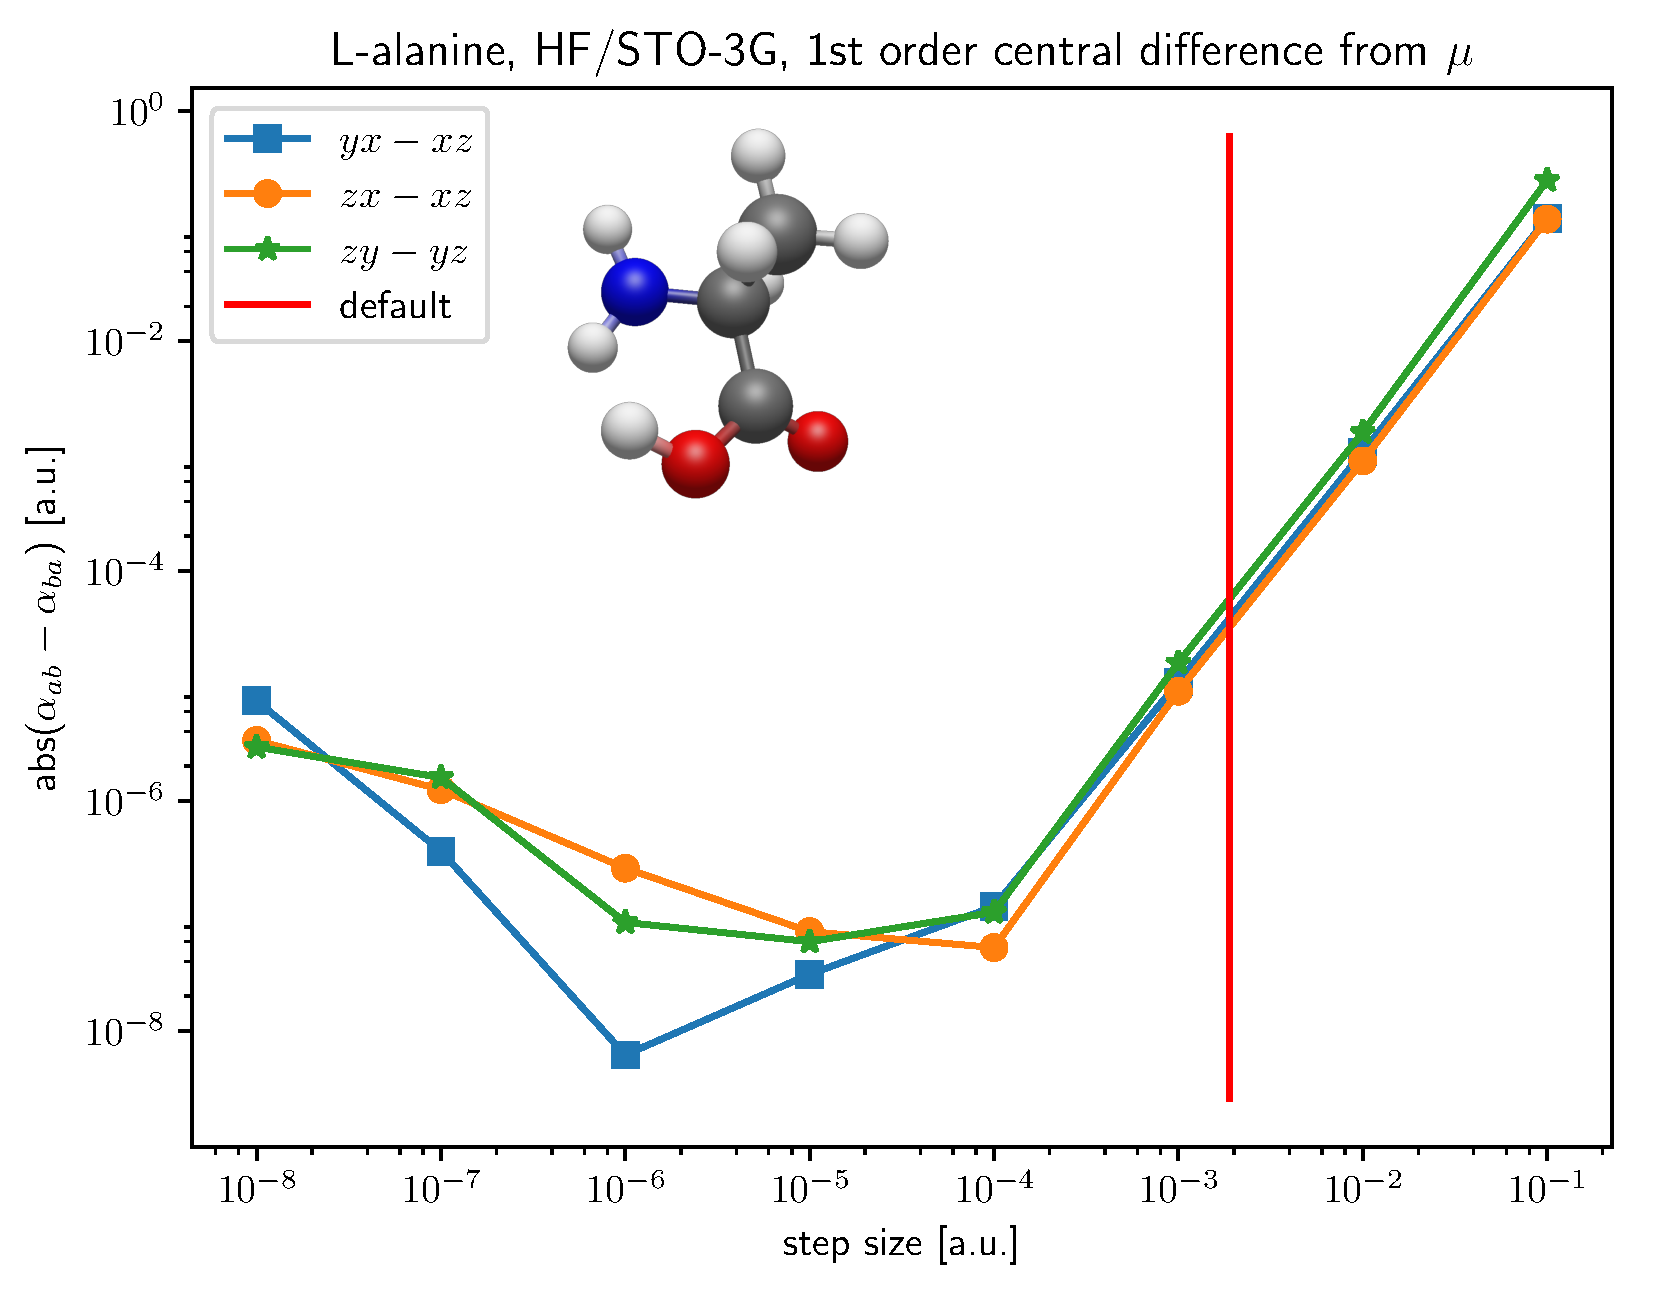
\includegraphics[width=\textwidth]{./diff_overlay.pdf}
  \caption[Asymmetry in the 1st-order finite-difference polarizability]{Effect of numerical noise on the off-diagonal matrix elements of the polarizability tensor. Nonzero differences indicate asymmetry, and the polarizability tensor is supposed to be symmetric. The red bar indicates the default step size for the applied electric field in \qchem{} 5.1, set at \SI{1.88973E-05}{\au}.\label{fig:finite-difference-numerical-noise}}
\end{figure}

\subsection{\texorpdfstring{\href{https://chemistry.stackexchange.com/q/89831/194}{\color{black}{Analytic derivative theory}}}{Analytic derivative theory}}
\label{ssec:analytic-derivative-theory}

As mentioned in section~\ref{ssec:derivative-evaluation}, the first requirement for evaluating analytic energy derivatives is to form the necessary mathematical expression. In the most general case, there are both derivatives of the atomic orbital (AO) basis integrals themselves and of the density matrix, which leads to derivatives of the MO coefficients. To illustrate some of the mechanics of differentiation, consider the derivative of the MO-basis matrix representation of the electron-nuclear attraction operator \(\hat{V}_{eN}\) with respect to a nuclear coordinate \(X_{A}\), which is a term needed for the molecular gradient:
\begin{align}
  \label{eq:yamaguchi-3.80}\tag{Yamaguchi eq. 3.80}
  \frac{\partial V_{ij}}{\partial X_{A}} &= \frac{\partial}{\partial X_{A}} \left( \sum_{\mu\nu}^{\text{AO}} C_{\mu i} C_{\nu j} V_{\mu\nu} \right) \\
  \label{3.81}\tag{Yamaguchi eq. 3.81}
                                         &= \sum_{\mu\nu}^{\text{AO}} \left( \frac{\partial C_{\mu i}}{\partial X_{A}} C_{\nu j} V_{\mu\nu} + C_{\mu i} \frac{\partial C_{\nu j}}{\partial X_{A}} V_{\mu\nu} + C_{\mu i} C_{\nu j} \frac{\partial V_{\mu\nu}}{\partial X_{A}} \right),
\end{align}
where the third (last) term is the true AO integral derivative, and the first two terms, the MO coefficient derivatives, come from differentiating the density matrix, which is defined as
\begin{equation}
  \label{eq:density-matrix}
  P_{\mu\nu}^{\text{RHF}} = \sum_{i}^{\text{d.o.}} C_{\mu i} C_{\nu i}
\end{equation}
in the AO basis.

The AO integral derivative can be further expanded. Using \(\mu,\nu\) rather than \(\chi_{\mu},\chi_{\nu}\) so they refer to both AO basis functions \emph{and} their matrix indices,
\begin{align}
  \tag{Yamaguchi eq. 3.24}
  \frac{\partial V_{\mu\nu}}{\partial X_{A}} &= \frac{\partial}{\partial X_{A}} \Braket{ \mu \left| \hat{V} \right| \nu } \\
  \label{3.25}\tag{Yamaguchi eq. 3.25}
                                             &= \Braket{ \frac{\partial \mu}{\partial X_{A}} \left| \hat{V} \right| \nu } + \Braket{ \mu \left| \frac{\partial \hat{V}}{\partial X_{A}} \right| \nu } + \Braket{ \mu \left| \hat{V} \right| \frac{\partial \nu}{\partial X_{A}} },
\end{align}
where the first and third terms are derivatives of basis functions and the second term is a derivative of the operator itself. Although AO integral derivatives are a necessary component of most derivative expressions, they do not play a direct role in response equations, and do not need to be discussed further.

It is convenient to rewrite the MO coefficient derivatives,
\begin{equation}
  \tag{Yamaguchi eq. 3.7}
  \frac{\partial C_{\mu i}}{\partial X_{A}} = \sum_{m}^{\text{MO}} U_{mi}^{X_{A}} C_{\mu m},
\end{equation}
where the index \(m\) runs over all occupied and unoccupied/virtual MOs. Although \(X_{A}\) is being used for the perturbation, all parts of this derivation hold for any general perturbation. The key insight is that the effect of a perturbation on the MO coefficients can be written as the contraction of the unmodified MO coeffcients with a unitary matrix describing single-particle excitations from occupied to virtual MOs, as well as deexcitations from virtual to occupied MOs. In matrix form, this is
\begin{equation}
  \label{eq:mo-coefficient-derivatives}
  \mathbf{C}^{(X_{A})} = \mathbf{C}^{(0)} \left( \mathbf{U}^{(X_{A})} \right)^{T},
\end{equation}
where the dimension of \(\mathbf{U}\) is \([N_{\text{orb}}, N_{\text{orb}}]\).

Now consider the derivatives of the MO coefficients/density matrix in the context of the \hf{} equations. Starting from the restricted \hf{} electronic energy expression,\footnote{\label{foot:hf-basics}\(\mu,\nu,\lambda,\sigma,\dots\) are AO indices, \(i,j,k,l,\dots\) are occupied MO indices, and \(p,q,r,s,\dots\) are general MO indices. \(\left(\hat{h} = \hat{H}^{\text{core}} \right) \equiv \hat{T}_{e} + \hat{V}_{Ne}\) is the one-electron core Hamiltonian operator, which itself is the sum of the electronic kinetic energy and electron-nuclear attraction energy operators, here in matrix representation, similar to \eqref{eq:yamaguchi-3.80}. \((pq|rs)\) is an MO-basis two-electron (repulsion) integral in Mulliken notation (see Table 2.2 of Ref.~\parencite{szabo1989modern}).}
\begin{equation}
  \label{eq:yamaguchi-4.1}\tag{Yamaguchi eq. 4.1}
  E_{\text{elec}}^{\text{RHF}} = 2 \sum_{i}^{\text{d.o.}} h_{ii} + \sum_{ij}^{\text{d.o.}} \left\{ 2(ii|jj) - (ij|ij) \right\},
\end{equation}
the first derivative with respect to a nuclear displacement \(X_{A}\) is\footnote{Additionally, see section C.3 of \szabo{}\cite{szabo1989modern} and Ref.~\parencite{Pople1979}.}
\begin{equation}
  \label{eq:yamaguchi-4.21}\tag{Yamaguchi eq. 4.21}
  \frac{\partial E_{\text{elec}}^{\text{RHF}}}{\partial X_{A}} = 2 \sum_{i}^{\text{d.o.}} h_{ii}^{X_{A}} + \sum_{ij}^{\text{d.o.}} \left\{ 2(ii|jj)^{X_{A}} - (ij|ij)^{X_{A}} \right\} - 2 \sum_{i}^{\text{d.o.}} S_{ii}^{X_{A}} \epsilon_{i},
\end{equation}
where terms with the superscript \(X_{A}\) indicate the a derivative of only the AO term.

Notice that the MO coefficient derivatives do not appear in the final HF gradient expression. They disappear due to Wigner's \(2n + 1\) rule. From page 25 of Ref.~\parencite{Yamaguchi1994}:
\begin{quote}
  When the wavefunction is determined up to the \(n\)th order, the expectation value (electronic energy) of the the system is resolved, according to the results of perturbation theory, up to the \((2n+1)\)st order. This principle is called Wigner's \(2n+1\) theorem\cite{doi:10.1063/1.1668053,EPSTEIN1980311}.
\end{quote}
More explicitly, we have the zeroth-order wavefunction, so we must be able to calculate the first-order correction to the energy. Worded differently, any first derivative of the energy can be calculated without differentiating MO coefficients, which is only required for second derivatives, such as the molecular Hessian or the dipole polarizability.

Differentiating \eqref{eq:yamaguchi-4.1} with respect to \(X_{A}\) and collecting terms with \(\mathbf{U}\) gives
\begin{equation}
  \label{4.16}\tag{Yamaguchi eq. 4.16}
  \frac{\partial E_{\text{elec}}^{\text{RHF}}}{\partial X_{A}} = 2 \sum_{i}^{\text{d.o.}} h_{ii}^{X_{A}} + \sum_{ij}^{\text{d.o.}} \left\{ 2(ii|jj)^{X_{A}} - (ij|ij)^{X_{A}} \right\} + 4 \sum_{m}^{\text{all}} \sum_{i}^{\text{d.o.}} U_{mi}^{X_{A}} F_{im},
\end{equation}
where the Fock matrix is defined as
\begin{equation}
  \label{eq:yamaguchi-4.6} \tag{Yamaguchi eq. 4.6}
  \begin{aligned}
    F_{pq} &= h_{pq} + \sum_{k}^{\text{d.o.}} \left\{ 2(pq|kk) - (pk|qk) \right\} \\
    &= h_{pq} + 2J_{pq} - K_{pq},
  \end{aligned}
\end{equation}
and the Coulomb and exchange matrices \(\mathbf{J}\) and \(\mathbf{K}\) have also been introduced. Using the RHF variational conditions, the Fock matrix from a converged calculation is diagonal in the MO basis, corresponding to the MO energies
\begin{equation}
  F_{pq} = \delta_{pq} \epsilon_{pq}, \tag{Yamaguchi eq. 4.7}
\end{equation}
so \eqref{4.16} simplifies to
\begin{equation}
  \frac{\partial E_{\text{elec}}^{\text{RHF}}}{\partial X_{A}} = 2 \sum_{i}^{\text{d.o.}} h_{ii}^{X_{A}} + \sum_{ij}^{\text{d.o.}} \left\{ 2(ii|jj)^{X_{A}} - (ij|ij)^{X_{A}} \right\} + 4 \sum_{m}^{\text{all}} \sum_{i}^{\text{d.o.}} U_{mi}^{X_{A}} \epsilon_{im}, \tag{Yamaguchi eq. 4.17 modified}
\end{equation}
which can be further simplified as
\begin{equation}
  \frac{\partial E_{\text{elec}}^{\text{RHF}}}{\partial X_{A}} = 2 \sum_{i}^{\text{d.o.}} h_{ii}^{X_{A}} + \sum_{ij}^{\text{d.o.}} \left\{ 2(ii|jj)^{X_{A}} - (ij|ij)^{X_{A}} \right\} + 4 \sum_{i}^{\text{d.o.}} U_{ii}^{X_{A}} \epsilon_{ii}. \tag{Yamaguchi eq. 4.17}
\end{equation}

Now one of the most important tricks in quantum chemistry is used. Given the orthonormality of the MOs,
\begin{equation}
S_{pq} = \delta_{pq}, \tag{Yamaguchi eq. 3.44}
\end{equation}
we must have (see \autoref{foot:overset})
\begin{equation}
  \label{eq:yamaguchi-3.45}\tag{Yamaguchi eq. 3.45}
  \frac{\partial S_{pq}}{\partial X_{A}} \overset{!}{=} 0.
\end{equation}
Expanding the left-hand side of \eqref{eq:yamaguchi-3.45} in a manner identical to \eqref{3.81} gives
\begin{align*}
\frac{\partial S_{pq}}{\partial X_{A}} &= \sum_{\mu\nu}^{\text{AO}} C_{\mu p} C_{\mu q} \frac{\partial S_{\mu\nu}}{\partial X_{A}} + \sum_{m}^{\text{all}} \left( U_{mp}^{X_{A}} S_{mq} + U_{mq}^{X_{A}} S_{pm} \right) \tag{Yamaguchi eqs. 3.40 + 3.43} \\
                                       &= S_{pq}^{X_{A}} + \sum_{m}^{\text{all}} \left( U_{mp}^{X_{A}} S_{mq} + U_{mq}^{X_{A}} S_{pm} \right). \tag{Yamaguchi eq. 3.43}
\end{align*}
The sum over all MOs can be eliminated by reusing the orthonormality condition, so in the first term \(m \overset{!}{=} q\) and for the second term \(m \overset{!}{=} p\), and the overlap matrix in the MO basis is unity for those terms, giving
\begin{equation}
  \label{eq:yamaguchi-3.46} \tag{Yamaguchi eq. 3.46}
  \frac{\partial S_{pq}}{\partial X_{A}} = S_{pq}^{X_{A}} + U_{qp}^{X_{A}} + U_{pq}^{X_{A}} \overset{!}{=} 0.
\end{equation}

Recognizing that we only need diagonal terms, this can be rewritten as
\begin{equation}
  \label{eq:yamaguchi-4.20} \tag{Yamaguchi eq. 4.20}
  U_{pp}^{X_{A}} = -\frac{1}{2} S_{pp}^{X_{A}},
\end{equation}
which is then plugged back into the first derivative expression to give
\begin{align*}
  \frac{\partial E_{\text{elec}}^{\text{RHF}}}{\partial X_{A}} &= 2 \sum_{i}^{\text{d.o.}} h_{ii}^{X_{A}} + \sum_{ij}^{\text{d.o.}} \left\{ 2(ii|jj)^{X_{A}} - (ij|ij)^{X_{A}} \right\} + 4 \sum_{i}^{\text{d.o.}} \left( -\frac{1}{2} S_{ii}^{X_{A}} \right) \epsilon_{ii} \\
                                                  &= 2 \sum_{i}^{\text{d.o.}} h_{ii}^{X_{A}} + \sum_{ij}^{\text{d.o.}} \left\{ 2(ii|jj)^{X_{A}} - (ij|ij)^{X_{A}} \right\} - 2 \sum_{i}^{\text{d.o.}} S_{ii}^{X_{A}} \epsilon_{ii}. \label{eq:yamaguchi-4.21-rederived}\tag{Yamaguchi eq. 4.21 [rederived]}
\end{align*}

Since is it almost always advantageous to avoid MO transformations and work in the AO basis, the last term can be rewritten
\begin{equation}
  \tag{Yamaguchi eq. 4.24}
  \begin{aligned}
    \sum_{i}^{\text{d.o.}} S_{ii}^{X_{A}} \epsilon_{ii} &= \sum_{i}^{\text{d.o.}} \sum_{\mu\nu}^{\text{AO}} C_{\mu i} C_{\mu i} \frac{\partial S_{\mu\nu}}{\partial X_{A}} \epsilon_{ii} \\
    &= \sum_{i}^{\text{d.o.}} \sum_{\mu\nu}^{\text{AO}} C_{\mu i} C_{\mu i} \epsilon_{ii} S_{\mu\nu}^{X_{A}} \\
    &= \sum_{\mu\nu}^{\text{AO}} W_{\mu\nu} S_{\mu\nu}^{X_{A}}
  \end{aligned}
\end{equation}
to use the energy-weighted density matrix \(\mathbf{W}\), also sometimes called \(\mathbf{Q}\):\footnote{The convention in \szabo{} is to absorb the RHF factor of 2 into the density matrix, which is not done here.}
\begin{equation}
  \label{eq:szabo-c12}
  \tag{\szabo{} eq. C.12}
  \frac{\partial E_{\text{elec}}^{\text{RHF}}}{\partial X_{A}} = 2 \sum_{\mu\nu}^{\text{AO}} P_{\mu\nu} h_{\mu\nu}^{X_{A}} + \sum_{\mu\nu\lambda\sigma}^{\text{AO}} P_{\mu\nu}P_{\lambda\sigma} \left\{ 2(\mu\nu|\lambda\sigma)^{X_{A}} - (\mu\lambda|\nu\sigma)^{X_{A}} \right\} - 2 \sum_{\mu\nu}^{\text{AO}} Q_{\mu\nu} S_{\mu\nu}^{X_{A}} + V_{NN}^{X_{A}}
\end{equation}

Again, the elimination of the \(\mathbf{U}\) matrix is one of the most important results in quantum chemistry, as it means the coupled-perturbed SCF equations described \hyperlink{text:response-equation-description}{previously} do not need to be solved for first derivatives of SCF wavefunctions. This is why density or MO coefficient derivatives are not present in the gradient expression.

Differentiation of \eqref{eq:yamaguchi-4.21} once more with respect to another nuclear displacement \(Y_{B}\) is
\begin{equation}
  \label{eq:yamaguchi-4.54-and-4.55-and-3.127}\tag{Yamaguchi eqs. 4.54, 4.55, 3.127}
  \begin{aligned}
    \frac{\partial^{2} E_{\text{tot}}^{\text{RHF}}}{\partial X_{A} \partial Y_{B}} &= 2 \sum_{i}^{\text{d.o.}} h_{ii}^{X_{A}Y_{B}} + \sum_{ij}^{\text{d.o.}} \left\{ 2(ii|jj)^{X_{A}Y_{B}} - (ij|ij)^{X_{A}Y_{B}} \right\} \\
    &- 2 \sum_{i}^{\text{d.o.}} S_{ii}^{X_{A}Y_{B}} \epsilon_{i} - 2 \sum_{i}^{\text{d.o.}} \sum_{p}^{\text{all}} \left\{ U_{ip}^{X_{A}}U_{ip}^{Y_{B}} + U_{ip}^{Y_{B}}U_{ip}^{X_{A}} - S_{ip}^{X_{A}}S_{ip}^{Y_{B}} - S_{ip}^{Y_{B}}S_{ip}^{X_{A}} \right\} \epsilon_{i} \\
    &+ 4 \sum_{p}^{\text{all}} \sum_{i}^{\text{d.o.}} \left( U_{pi}^{Y_{B}} F_{pi}^{X_{A}} + U_{pi}^{X_{A}} F_{pi}^{Y_{B}} \right) + 4 \sum_{p}^{\text{all}} \sum_{i}^{\text{d.o.}} U_{pi}^{X_{A}} U_{pi}^{Y_{B}} \epsilon_{p} \\
    &+ 4 \sum_{p}^{\text{all}} \sum_{i}^{\text{d.o.}} \sum_{q}^{\text{all}} \sum_{j}^{\text{d.o.}} U_{pi}^{X_{A}} U_{qj}^{Y_{B}} \left\{ 4(pi|qj) - (pq|ij) - (pj|iq) \right\} \\
    &- 3\left(X_{A}-X_{B}\right)\left(Y_{A}-Y_{B}\right)\frac{Z_{A}Z_{B}}{R_{AB}^{5}},
  \end{aligned}
\end{equation}
where the nucleus-nucleus repulsion energy derivative is included for completeness. This is the final expression for the molecular Hessian\footnote{Not mass-weighted.} derived in \eqref{eq:hooke_derivation_3}. From here and Table~\ref{tutorial:tab:wigner}, we can see that evaluating the \(\mathbf{U}\) matrices (forming derivatives of the MO coefficients) is unavoidable.

However, the case of the molecular Hessian is a general one, because the AOs are perturbation-dependent: for a fixed electron position, the amplitude of a basis function will change if it moved, and they are typically atom-centered. In the case that the basis set is \textit{not} perturbation dependent, as is most often in the case in electric field perturbations\footnote{See Ref.~\parencite{doi:10.1021/j100074a008} for a discussion of using electric field-dependent functions.}, \eqref{eq:yamaguchi-4.54-and-4.55-and-3.127} reduces to
\begin{equation}
  \label{eq:yamaguchi-17.54} \tag{Yamaguchi eq. 17.54}
  \frac{\partial^{2} E_{\text{tot}}^{\text{RHF}}}{\partial F_{\alpha} \partial F_{\beta}} = -4 \sum_{a}^{\text{virt}} \sum_{i}^{\text{d.o.}} U_{ai}^{F_{\beta}} h_{ai}^{F_{\alpha}},
\end{equation}
where \(\frac{\partial^{2} E_{\text{tot}}^{\text{RHF}}}{\partial F_{\alpha} \partial F_{\beta}}\) is the \(\alpha\beta\)-component of the static polarizability tensor \eqref{eq:polarizability-derivative-definition}, and the one-electron term \(h_{ai}^{F_{\alpha}}\) is the \(\alpha\)-component of the dipole operator in the occupied-virtual MO basis (the \emph{property gradient}, see the \(\mathbf{P}/\mathbf{Q}\) matrix elements in section~\ref{ssec:linear-response-formalism} and line~\ref{line:form_polarizability}). This specific term originates from the Fock matrix derivatives on line three, as the complete Hamiltonian now includes the perturbation (see \eqref{eq:perturbed-hamiltonian}), which is the only term that survives the differentiation. In general, when the AO basis is perturbation independent, the energy derivative with respect to two arbitrary perturbations \(\lambda\) and \(\theta\) can be written as\cite{NEESE2009526}
\begin{equation}
  \label{eq:neese-77} \tag{Neese eq. 77}
  \frac{\partial^{2} E}{\partial \lambda \partial \theta} = \sum_{\mu\nu} \left( P_{\mu\nu} \frac{\partial^{2} h_{\mu\nu}}{\partial \lambda \partial \theta} + \frac{\partial P_{\mu\nu}}{\partial \theta} \frac{\partial h_{\mu\nu}}{\partial \lambda} \right),
\end{equation}
where the first term is evaluated as an expectation value and the second term requires solution of the response equations. The derivative of the density matrix is related to the \(\mathbf{U}\) matrices via\footnote{\eqref{eq:neese-77} is for real perturbations; in the case of imaginary perturbations, the sum changes to a difference.}
\begin{equation}
  \frac{\partial \mathbf{P}}{\partial \theta} = \mathbf{C}^{(0)} \left( \mathbf{C}^{(\theta)} \right)^{T} + \mathbf{C}^{(\theta)} \left( \mathbf{C}^{(0)} \right)^{T}
\end{equation}
and \eqref{eq:mo-coefficient-derivatives}.

The form of \eqref{eq:yamaguchi-17.54} and \eqref{eq:neese-77} as shown above should make it clear that for a second derivative of an HF wavefunction, only one set of \(\mathbf{U}\) matrices is needed. This leads to a potential computational savings. Considering the IR intensities \(\frac{d^{2}E}{dX_{A}dF_{\alpha}}\), calculating \(\frac{d}{d X_{A}} \left(\mu_{\alpha}\right)\) would require \(3N\) \(\mathbf{U}\) matrices (one for each nuclear displacement), but using \eqref{eq:youngs-theorem} to calculate \(\frac{d}{d F_{\alpha}} \left(\frac{d E}{d X_{A}}\right)\) would only require \(3\) \(\mathbf{U}\) matrices (one for each external field component).

\subsection{Perturbation theory}
\label{ssec:perturbation-theory}

In Rayleigh\textendash{}\schrod{} perturbation theory\footnote{See \szabo{}\cite{szabo1989modern} page 322; identical notation is followed throughout, except the summation index \(n\) is generally replaced with \(k\).}, the exact Hamiltonian \(\hat{H}\) of a system under an applied perturbation \(\hat{V}\) can be written as
\begin{equation}
  \label{eq:perturbed-hamiltonian}
  \hat{H} = \hat{H}^{(0)} + \lambda\hat{V},
\end{equation}
where \(\hat{H}^{(0)}\) is the Hamiltonian in the absence of the perturbation and \(\lambda \in [0,1]\) controls the strength of the perturbation. Note that it is not yet necessary to specify the exact form of \(\hat{V}\). The main assumption in perturbation theory, worded in two ways, is that the unperturbed Hamiltonian is an acceptable approximation to the exact Hamiltonian, and the perturbation is small. This assumption allows for a power (Maclaurin) series expansion of the wavefunction \(\ket{\Psi_{i}}\) and its energy \(\mathcal{E}_{i}\) for a given state \(i\), where increasing orders account for better approximations to the exact (perturbed) energy:\footnote{While one hopes the series is convergent, it is often not the case, so the series is often truncated at the second-order correction to the energy, which may still be useful. See Ref.~\parencite{NOBES1987481} for a series convergence study. It is unclear if the same issue exists when \(\hat{V}\) corresponds to an operator other than \(\hat{V}_{ee}\), such as for external fields.}
\begin{align}
  \label{eq:expansion-wavefunction}
  \ket{\Psi_{i}} &= \ket{\psi_{i}^{(0)}} + \lambda\ket{\psi_{i}^{(1)}} + \lambda^{2}\ket{\psi_{i}^{(2)}} + \dots \\
  \label{eq:expansion-energy}
  \mathcal{E}_{i} &= E_{i}^{(0)} + \lambda E_{i}^{(1)} + \lambda^{2} E_{i}^{(2)} + \dots
\end{align}

Combining \eqref{eq:perturbed-hamiltonian}, \eqref{eq:expansion-wavefunction}, and \eqref{eq:expansion-energy} into the \schrod{} equation,
\begin{equation}
  \label{eq:schrodinger-equation}
  \hat{H}\ket{\Psi_{i}} = \mathcal{E}_{i}\ket{\Psi_{i}},
\end{equation}
gives
\begin{equation}
  \label{eq:expansion-schrodinger}
  \begin{aligned}
    \left( \hat{H}^{(0)} + \lambda\hat{V} \right) &\left[ \ket{\psi_{i}^{(0)}} + \lambda\ket{\psi_{i}^{(1)}} + \lambda^{2}\ket{\psi_{i}^{(2)}} + \dots \right] \\
    &= \left[ E_{i}^{(0)} + \lambda E_{i}^{(1)} + \lambda^{2} E_{i}^{(2)} + \dots \right] \left[ \ket{\psi_{i}^{(0)}} + \lambda\ket{\psi_{i}^{(1)}} + \lambda^{2}\ket{\psi_{i}^{(2)}} + \dots \right],
  \end{aligned}
\end{equation}
where the \(\{\lambda\}\) are now also useful for collecting terms of like orders. The zeroth-order terms give the \schrod{} equation for the unperturbed energy,
\begin{equation}
  \label{eq:unperturbed-energy}
  \hat{H}^{(0)} \ket{\psi_{i}^{(0)}} = E_{i}^{(0)} \ket{\psi_{i}^{(0)}},
\end{equation}
but equating all terms that are first order in \(\lambda\) on both sides gives
\begin{equation}
  \label{eq:first-order-terms}
  \hat{H}^{(0)} \ket{\psi_{i}^{(1)}} + \hat{V} \ket{\psi_{i}^{(0)}} = E_{i}^{(0)} \ket{\psi_{i}^{(1)}} + E_{i}^{(1)} \ket{\psi_{i}^{(0)}},
\end{equation}
where \(\lambda\) has been dropped for readability since it is present in front of each term. \eqref{eq:first-order-terms} can be simplified through integration using the bra \(\bra{\psi_{i}^{(0)}}\), which does not change the order from \(\lambda^{1}\):
\begin{equation}
  \label{eq:first-order-terms-bra}
  \begin{aligned}
    \bra{\psi_{i}^{(0)}} \left( \hat{H}^{(0)} \ket{\psi_{i}^{(1)}} + \hat{V} \ket{\psi_{i}^{(0)}} \right) &= \bra{\psi_{i}^{(0)}} \left( E_{i}^{(0)} \ket{\psi_{i}^{(1)}} + E_{i}^{(1)} \ket{\psi_{i}^{(0)}} \right) \\
    \braket{\psi_{i}^{(0)} | \hat{H}^{(0)} | \psi_{i}^{(1)}} + \braket{\psi_{i}^{(0)} | \hat{V} | \psi_{i}^{(0)}} &= \braket{\psi_{i}^{(0)} | E_{i}^{(0)} | \psi_{i}^{(1)}} + \braket{\psi_{i}^{(0)} | E_{i}^{(1)} | \psi_{i}^{(0)}} \\
    &= E_{i}^{(0)} \braket{\psi_{i}^{(0)} | \psi_{i}^{(1)}} + E_{i}^{(1)} \braket{\psi_{i}^{(0)} | \psi_{i}^{(0)}}.
  \end{aligned}
\end{equation}

It is now important to know what orthonormality conditions exist between the set of all corrected states \(\left\{\ket{\psi_{i}^{(n)}}\right\}\). For the unperturbed state, which is usually the \hf{} ground state,
\begin{equation}
  \label{eq:hf-normalization}
  \braket{\psi_{i}^{(0)}|\psi_{i}^{(0)}} = 1,
\end{equation}
and the choice of \emph{intermediate normalization} is made,
\begin{equation}
  \label{eq:intermediate-normalization}
  \braket{\psi_{i}^{(0)}|\Psi_{i}} \overset{!}{=} 1,
\end{equation}
which upon expanding the ket using \eqref{eq:expansion-wavefunction} leads to
\begin{equation}
  \label{eq:intermediate-normalization-single}
  \braket{\psi_{i}^{(0)}|\psi_{i}^{(n)}} = 0
\end{equation}
for any correction state where \(n > 0\). Returning to \eqref{eq:first-order-terms-bra}, this first allows for simplification of the right-hand side,
\begin{equation}
  \label{eq:first-order-terms-first-simplification}
  \begin{aligned}
    \braket{\psi_{i}^{(0)} | \hat{H}^{(0)} | \psi_{i}^{(1)}} + \braket{\psi_{i}^{(0)} | \hat{V} | \psi_{i}^{(0)}} &= E_{i}^{(0)} \Ccancelto[carmine]{0}{\braket{\psi_{i}^{(0)} | \psi_{i}^{(1)}}} + E_{i}^{(1)} \Ccancelto[Green]{1}{\braket{\psi_{i}^{(0)} | \psi_{i}^{(0)}}} \\
    &= E_{i}^{(1)},
  \end{aligned}
\end{equation}
and the first term on the left-hand side can be simplified using the hermiticity of the Hamiltonian followed by \eqref{eq:intermediate-normalization-single},
\begin{equation}
  \label{eq:hermiticity}
  \begin{aligned}
    \braket{\psi_{i}^{(0)} | \hat{H}^{(0)} | \psi_{i}^{(1)}} &= \braket{\psi_{i}^{(1)} | \hat{H}^{(0)} | \psi_{i}^{(0)}}^{*} \\
    &= \braket{\psi_{i}^{(1)} | E_{i}^{(0)} | \psi_{i}^{(0)}}^{*} \\
    &= E_{i}^{(0)} \braket{\psi_{i}^{(1)} | \psi_{i}^{(0)}}^{*} \\
    &= E_{i}^{(0)} \Ccancelto[carmine]{0}{\braket{\psi_{i}^{(0)} | \psi_{i}^{(1)}}} \\
    &= 0.
  \end{aligned}
\end{equation}
The final form of \eqref{eq:first-order-terms-bra} is now
\begin{equation}
  \label{eq:first-order-terms-final}
  \braket{\psi_{i}^{(0)} | \hat{V} | \psi_{i}^{(0)}} = E_{i}^{(1)},
\end{equation}
revealing that the first-order correction to the energy is the expectation value of the perturbation operator over the zeroth-order wavefunction. For context, when using perturbation theory to approximate the correlation energy of system on top of the mean-field wavefunction, \(\hat{V} \equiv \hat{V}_{ee} = \frac{1}{|\vec{r}_{1} - \vec{r}_{2}|} = \frac{1}{r_{12}}\), the electron-electron repulsion operator. However, the perturbation operator may be any one- or two-electron operator, and \eqref{eq:first-order-terms-final} is exact as long as \(\ket{\psi_{i}^{(0)}}\) is a variationally-optimized state\footnote{\hf{} and most density functional approximations that do not contain a perturbative correction (such as double hybrids) satisfy this criterion. Additionally, it is important for ALMO-EDA, where the polarized but CT-disallowed intermediate state \(\ket{\psi_{\text{pol}}}\) is variational, but the frozen density state \(\ket{\psi_{\text{frz}}}\) is \emph{not}. All the work found in chapter~\ref{ch:paper_04} starts from \(\ket{\psi_{\text{pol}}}\), so the use of a Lagrangian to account for orbital relaxation (leading to additional terms) is unnecessary.}. The key insight is that to calculate the first-order correction to the energy, only the zeroth-order wavefunction is required. This means that if \(\hat{V}\) is replaced with an operator related to a molecular property, it can be calculated as an expectation value without needing the perturbed wavefunction. This is the same result as in \eqref{eq:yamaguchi-4.21}, and resembles the result of the \hefe{} theorem when the AO basis is not dependent on the perturbation.

The generalization of \eqref{eq:first-order-terms-final} is that for \(n > 0\), the \(n\)th order correction to the energy is given by
\begin{equation}
  \label{eq:general-energy-correction}
  E_{i}^{(n)} = \braket{\psi_{i}^{(0)}|\hat{V}|\psi_{i}^{(n-1)}},
\end{equation}
so to find the second-order correction to the energy, the first-order correction to the wavefunction is required. The general rule is that given the \(n\)th order correction to the wavefunction, the \(2n+1\)th order correction to the energy can be calculated. This is known as Wigner's \(2n+1\) rule (see section~\ref{wigners-2n-1-rule}). From \eqref{eq:general-energy-correction}, the first form of the second-order correction is
\begin{equation}
  \label{eq:second-order-correction-first-form}
  E_{i}^{(2)} = \braket{\psi_{i}^{(0)}|\hat{V}|\psi_{i}^{(1)}},
\end{equation}
where the problem now becomes the calculation of the perturbed wavefunction \(\ket{\psi_{i}^{(1)}}\). The strategy is to expand it as a linear combination of eigenfunctions of \(\hat{H}^{(0)}\) that are orthogonal to the unperturbed state (in line with \eqref{eq:intermediate-normalization-single}),
\begin{equation}
  \label{eq:orthogonal-to-reference-state}
  \braket{k|\psi_{i}^{(0)}} \overset{!}{=} 0,
\end{equation}
and form a complete orthonormal set \(\left\{\ket{\psi_{k}^{(0)}}\right\} \equiv \left\{\ket{k}\right\}\),
\begin{equation}
  \label{eq:orthonormal-eigenfunction-expansion}
  \ket{\psi_{i}^{(1)}} = \sum_{k} c_{k}^{(1)} \ket{k},
\end{equation}
leading to
\begin{equation}
  \label{eq:coefficient-selection}
  \braket{k|\psi_{i}^{(1)}} = c_{k}^{(1)}.
\end{equation}
Using \eqref{eq:intermediate-normalization-single} and the fact that the set \(\{\ket{k}\}\) is complete, the resolution of the identity can be inserted:
\begin{equation}
  \label{eq:resolution-of-the-identity}
  \ket{\psi_{i}^{(1)}} = \sum_{k} \ket{k} \braket{k|\psi_{i}^{(1)}}
\end{equation}

To calculate the first-order correction to the wavefunction, first rearrange \eqref{eq:first-order-terms} to collect all terms with the same ket,
\begin{equation}
  \label{eq:first-order-terms-group-kets}
  ( E_{i}^{(0)} - \hat{H}^{(0)} ) \ket{\psi_{i}^{(1)}} = ( \hat{V} - E_{i}^{(1)} ) \ket{\psi_{i}^{(0)}},
\end{equation}
and multiply \eqref{eq:first-order-terms-group-kets} on the left with \(\bra{k}\) to give
\begin{equation}
  \label{eq:first-order-terms-group-kets-cancelled}
  E_{i}^{(0)} \braket{k|\psi_{i}^{(1)}} - \braket{k|\hat{H}^{(0)}|\psi_{i}^{(1)}} = \braket{k|\hat{V}|\psi_{i}^{(0)}} - E_{i}^{(1)} \Ccancelto[carmine]{0}{\braket{k|\psi_{i}^{(0)}}},
\end{equation}
where the last term cancels due to \(\braket{a|b} = \delta_{ab}, \{a,b\}\in k\), and \(\ket{k} \neq \ket{\psi_{i}^{(0)}}\) from \eqref{eq:orthogonal-to-reference-state}. To deal with the second term, use \eqref{eq:orthonormal-eigenfunction-expansion}, canceling terms again due to orthonormality, and finally inserting \eqref{eq:coefficient-selection}:
\begin{equation}
  \label{eq:something-something-expansion}
  \begin{aligned}
    \braket{k|\hat{H}^{(0)}|\psi_{i}^{(1)}} &= \bra{k} \hat{H}^{(0)} | \left( \sum_{a} c_{a}^{(1)} \ket{a} \right) \\
      &= \bra{k} \hat{H}^{(0)}| \left( c_{a}^{(1)} \ket{a} + c_{b}^{(1)} \ket{b} + \dots + c_{k}^{(1)} \ket{k} + \dots \right) \\
      &= \bra{k} \left( E_{a}^{(0)} c_{a}^{(1)} \ket{a} + E_{b}^{(0)} c_{b}^{(1)} \ket{b} + \dots + E_{k}^{(0)} c_{k}^{(1)} \ket{k} + \dots \right) \\
      &= E_{a}^{(0)} c_{a}^{(1)} \Ccancelto[carmine]{0}{\braket{k|a}} + E_{b}^{(0)} c_{b}^{(1)} \Ccancelto[carmine]{0}{\braket{k|b}} + \dots + E_{k}^{(0)} c_{k}^{(1)} \Ccancelto[Green]{1}{\braket{k|k}} + \dots \\
      &= E_{k}^{(0)} c_{k}^{(1)} \\
      &= E_{k}^{(0)} \braket{k|\psi_{i}^{(1)}}.
    \end{aligned}
\end{equation}
Plugging \eqref{eq:something-something-expansion} back into \eqref{eq:first-order-terms-group-kets-cancelled} gives
\begin{align}
  \label{eq:szabo-ostlund-6.11}
  \left( E_{i}^{(0)} - E_{k}^{(0)} \right) \braket{k|\psi_{i}^{(1)}} &= \braket{k|\hat{V}|\psi_{i}^{(0)}} \\
  \label{eq:szabo-ostlund-6.11nl}
  \braket{k|\psi_{i}^{(1)}} &= \frac{\braket{k|\hat{V}|\psi_{i}^{(0)}}}{E_{i}^{(0)} - E_{k}^{(0)}},
\end{align}
which upon inserting into \eqref{eq:resolution-of-the-identity}, gives the final form of the first-order correction to the perturbed wavefunction:
\begin{equation}
  \label{eq:first-order-wavefunction}
  \ket{\psi_{i}^{(1)}} = \sum_{k\neq i} \ket{k} \frac{\braket{k|\hat{V}|\psi_{i}^{(0)}}}{E_{i}^{(0)} - E_{k}^{(0)}}.
\end{equation}
Inserting \eqref{eq:first-order-wavefunction} into \eqref{eq:second-order-correction-first-form} then gives the second-order correction to the perturbed energy:
\begin{equation}
  \label{eq:second-order-energy}
  \begin{aligned}
    E_{i}^{(2)} &= \bra{\psi_{i}^{(0)}} \hat{V} \left\{ \sum_{k\neq i} \ket{k} \frac{\braket{k|\hat{V}|\psi_{i}^{(0)}}}{E_{i}^{(0)} - E_{k}^{(0)}} \right\} \\
    &= \sum_{k \neq i} \frac{\braket{\psi_{i}^{(0)}|\hat{V}|k}\braket{k|\hat{V}|\psi_{i}^{(0)}}}{E_{i}^{(0)} - E_{k}^{(0)}}.
  \end{aligned}
\end{equation}
In the case where \(\hat{V}\) is operator with multiple components, such as the dipole operator in \eqref{eq:dipole-operator}, the energy becomes a rank-2 tensor, the polarizability matrix:
\begin{equation}
  \label{eq:static-polarizability-from-perturbation-theory}
  \alpha_{ab}= - \sum_{k \neq i} \frac{\braket{\psi_{i}^{(0)}|\hat{\mu}_{a}|k}\braket{k|\hat{\mu}_{b}|\psi_{i}^{(0)}}}{E_{i}^{(0)} - E_{k}^{(0)}}.
\end{equation} % \fxnote{TODO This expression is still incomplete regarding time-varying perturbations and mixed-operator properties.}
\eqref{eq:static-polarizability-from-perturbation-theory} is called a \emph{sum-over-states} expansion due to the explicit summation over the set of excited states \(\ket{\psi_{k}^{(0)}}\). Although the derivation assumes that all states are exact and the summation is infinite, the actual states are formed from the basis of excited Slater determinants using the converged SCF wavefunction as the reference state \(\ket{\psi_{i}^{(0)}}\).

\section{\texorpdfstring{\caps{Dynamic (frequency-dependent) response properties}}{Static (time-independent) response properties}}
\label{sec:dynamic-properties}

Up to this point, only static perturbations have been considered, where the strength of an applied field does not oscillate or vary with time. This is perfectly satisfactory for many properties, such as those that are intrinsic to the system or do not depend on field strength. For example, it does not make sense to have a field strength directly associated with a change in nuclear positions; this is not the same thing as having nuclear positions change in the presence of an applied field. Similarly, from Table~\ref{tab:gauss}, rotational and nuclear magnetic moments do not have a strength associated with them. This holds generally for ``internal'' perturbations. However, many non-linear optical processes in particular take advantage of oscillating fields, so frequency- or time-dependent molecular response properties must be calculable.

In order to deal with frequency-dependent response, a slightly different path must be taken, in part because the total energy of the system is no longer stationary with time, so energy derivatives as encountered in Section~\ref{ssec:analytic-derivative-theory} are not physically well-defined. There are numerous possible derivation frameworks which cannot be done justice here. Equivalent results arise from time-dependent perturbation theory, quasienergy derivatives\cite{Christiansen1998,gauss2000,C1CP21951K,Toulouse2015}, and the polarization propagator\cite{mcweeny1989methods}, to name a few. Ideally, there is a time-dependent extension of Section~\ref{ssec:series-expansion} that at some step allows for identification of coefficients in a series expansion with response functions. Similarly, in the static limit (\(\omega \rightarrow 0\)), results from analytic derivative theory should be recovered, making time-dependent response theory a more general framework for response properties. The following derivation is borrowed heavily from Ref.~\parencite{Toulouse2015}, with expansion using Ref.~\parencite{gauss2000}.

\subsection{Quasienergy derivatives}

The starting point is the now the time-dependent \schrod{} equation (TDSE),
\begin{equation}
  \label{eq:tdse}
  \hat{H}(t) \ket{\Psi(t)} = i\frac{\partial}{\partial t} \ket{\Psi(t)},
\end{equation}
which, unlike \eqref{eq:schrodinger-equation} does not have the energy on the right-hand side. It is useful to factor out the time-dependent phase of the wavefunction,
\begin{equation}
  \label{eq:phase-isolated-wavefunction} \tag{Toulouse eq. 48}
  \ket{\Psi(t)} = e^{-i\mathcal{F}(t)} \ket{\tilde{\Psi}(t)},
\end{equation}
where \(\Psi(t)\) is the original unfactored wavefunction, \(\mathcal{F}(t)\) is a phase factor, and \(\tilde{\Psi}(t)\) is the \emph{phase-isolated wavefunction}.\footnote{This notation is consistent with Ref.~\parencite{gauss2000}. In Ref.~\parencite{Toulouse2015}, \(\bar{\Psi}(t)\) is the total wavefunction and \(\Psi(t)\) is the phase-isolated wavefunction. In Ref.~\parencite{Christiansen1998}, \(\ket{\bar{0}}\) is the total wavefunction, \(\ket{\tilde{0}}\) is the phase-isolated wavefunction, and \(\ket{0}\) is the stationary wavefunction, recovered from \(\ket{\tilde{0}(t \rightarrow 0)}\).} Rearrange the TDSE \eqref{eq:tdse},
\begin{equation}
  \label{eq:tdse-rearranged} \tag{Toulouse eq. 47}
  \left[ \hat{H}(t) - i\frac{\partial}{\partial t} \right] \ket{\Psi(t)} = 0,
\end{equation}
and use the phase-isolated wavefunction\footnote{\(\dot{A}(t) = \mathrm{d}A(t)/\mathrm{d}t\)}
\begin{equation}
  \label{eq:phase-isolated-tdse} \tag{Toulouse eq. 49}
  \left[ \hat{H}(t) - i\frac{\partial}{\partial t} \right] \ket{\tilde{\Psi}(t)} = \dot{\mathcal{F}}(t) \ket{\tilde{\Psi}(t)},
\end{equation}
where \(\dot{\mathcal{F}}(t)\) now resembles the energy from the time-independent \schrod{} equation (TISE). This ``energy'' is still not stationary with time, however it will reappear later as part of a stationary theory.

Before going further, the Hamiltonian must be specified. The partitioning introduced in \eqref{eq:perturbed-hamiltonian} is modified:
\begin{equation}
  \label{eq:perturbed-hamiltonian-time-dependent}
  \hat{H}(t) = \hat{H}^{(0)} + \hat{V}(t),
\end{equation}
so that time-dependence is introduced only to the perturbation and not the standard molecular Hamiltonian.\footnote{Sometimes \(\hat{V}(t)\) is notated as \(\hat{H}'(t)\) or \(\hat{H}^{(1)}(t)\); all are equivalent as long as the perturbation and time partitioning in the full Hamiltonian are the same.} The prototypical perturbation usually represents an external electric field that is slowly turned on in order for the system to gradually respond and may oscillate with time at a characteristic frequency.\footnote{In the case that the response of the system is slower than the speed of which the perturbation is turned on, a different (undesirable) solution may be found if the perturbation is strong enough.} Representing the perturbation in terms of Fourier components,
\begin{equation}
  \label{eq:fourier-components} \tag{Toulouse eq. 46 [modified]}
  \hat{V}(t) = x_{1} \hat{B} e^{-i\omega t} + x_{2} \hat{A} e^{+i\omega t},
\end{equation} %TODO I am really not satisfied with this
shows that the perturbation, and therefore the Hamiltonian, is periodic in time (\(\hat{H}(t + T) = \hat{H}(t)\)) with a period of \(T = 2\pi/\omega\). Other perturbation shapes, such as step functions, can be represented using a more general form of \eqref{eq:fourier-components} with more Fourier components:
\begin{equation}
  \label{eq:general-fourier-components-gauss-106}\tag{Gauss eq. 106}
  \hat{V}(t) = \sum_{k=-N}^{N} e^{-i\omega_{k}t} \sum_{X} \epsilon_{X}(\omega_{k})\hat{X},
\end{equation}
where \(k\) is the Fourier component index, \(\omega_{k}\) are the frequencies, and \(\epsilon_{X}(\omega_{k})\) and \(\hat{X}\) are the corresponding perturbation strengths and operators. This gives the required integration bounds for \eqref{eq:phase-isolated-tdse}, leading to
\begin{equation}
  \label{eq:quasienergy} \tag{Toulouse eq. 50}
  \begin{aligned}
    \mathcal{Q} &= \frac{1}{T} \int_{0}^{T} \mathrm{d}t \, \dot{\mathcal{F}}(t) \\
    &= \frac{1}{T} \int_{0}^{T} \mathrm{d}t \, \frac{\bra{\tilde{\Psi}(t)} \left[ \hat{H}(t) - i\frac{\partial}{\partial t} \right] \ket{\tilde{\Psi}(t)}}{\braket{\tilde{\Psi}(t)|\tilde{\Psi}(t)}},
  \end{aligned}
\end{equation}
where \(\mathcal{Q}\) is the \emph{time-averaged quasienergy}. The second part of \eqref{eq:quasienergy} is the variational condition for \(\tilde{\Psi}(t)\), making \(\mathcal{Q}\) stationary with respect to fluctuations in \(\tilde{\Psi}(t)\). In the time-independent case, the quasienergy reduces to the (time-independent) energy, and the phase-isolated wavefunction reduces to the (time-independent) wavefunction.

The time-averaged quasienergy can now be expanded with respect to the perturbation parameters,
\begin{equation}
  \label{eq:quasienergy-expansion} \tag{Toulouse eq. 51}
  \mathcal{Q}(x_{1},x_{2}) = \mathcal{Q}^{(0)} + \mathcal{Q}^{(10)}x_{1} + \mathcal{Q}^{(01)}x_{2} + \frac{1}{2}\mathcal{Q}^{(20)}x_{1}^{2} + \mathcal{Q}^{(11)}x_{1}x_{2} + \frac{1}{2}\mathcal{Q}^{(02)}x_{2}^{2} + \dots,
\end{equation}
analogous to the series expansion in Section~\ref{ssec:series-expansion}. However, the expansion coefficients \(\partial^{n}\mathcal{Q}/\partial x^{n}\) are still not in a position to be directly calculable for an approximate theory due to the presence of the integral in \eqref{eq:quasienergy}, unlike in the static case, so the time-dependent theory must be further derived for exact states.

Using the time-dependent form of \eqref{eq:first-order-terms-final},
\begin{equation}
  \label{eq:quasienergy-10} \tag{Toulouse eq. 53}
  \begin{aligned}
    \mathcal{Q}^{(10)} &= \frac{1}{T} \int_{0}^{T} \mathrm{d}t \, \braket{\tilde{\Psi}_{0}|\hat{B}e^{-i\omega t}|\tilde{\Psi}_{0}} \\
    &= \braket{\tilde{\Psi}_{0}|\hat{B}|\tilde{\Psi}_{0}} \delta[\omega].
\end{aligned}
\end{equation}
The rule used in \eqref{eq:quasienergy-10} is
\begin{equation}
  \label{eq:kronecker-delta-frequencies}
  \frac{1}{T} \int_{0}^{T} \mathrm{d}t \, e^{-i\omega t} = \delta[\omega] =
  \begin{cases}
    \delta_{\omega,0} & |T| < \infty \\
    \delta(\omega) & T \rightarrow \infty
  \end{cases},
\end{equation}
where we define \(\delta[\omega]\) as the Kronecker delta for finite \(T\) and the Dirac delta for \(T \rightarrow \infty\). More explicitly, \(\delta[\omega = 0] = (1/T) \int_{0}^{T} \mathrm{d}t \, e^{0} = 1\). \(\delta[\omega \neq 0]\) would lead a non-zero value for exponential inside \eqref{eq:kronecker-delta-frequencies}, which when expanded as sines and cosines, gives rise to terms that are not physically admissible as Fourier components. The conclusion is that only static first-order properties are non-zero, where the physical intuition is that absorption or emission of a photon with \(\omega \neq 0\) would violate energy conservation. Using \eqref{eq:second-order-correction-first-form} and \eqref{eq:intermediate-normalization},
\begin{equation}
  \label{eq:quasienergy-20} \tag{Toulouse eq. 54}
  \mathcal{Q}^{(20)} = \frac{1}{T} \int_{0}^{T} \mathrm{d}t \, 2\braket{\tilde{\Psi}_{0}|\hat{B}e^{-i\omega t}|\tilde{\Psi}^{(10)}(t)},
\end{equation}
where the first-order wavefunction correction is (similar to \eqref{eq:orthonormal-eigenfunction-expansion})
\begin{equation}
  \label{eq:first-order-wavefunction-td} \tag{Toulouse eq. 55}
  \ket{\tilde{\Psi}^{(10)}(t)} = \sum_{n\neq 0} c_{n}^{(10)}(t) e^{-i\omega_{n0}t} \ket{\tilde{\Psi}_{n}},
\end{equation}
where \(\omega_{n0} = E_{n} - E_{0}\) are the unperturbed system excitation energies. The first-order wavefunction expansion coefficients are found similarly to \eqref{eq:coefficient-selection},
\begin{equation}
  \label{eq:56} \tag{Toulouse eq. 56}
  c_{n}^{(10)}(t) = -i \int_{-\infty}^{t} \mathrm{d}t' \, \braket{\tilde{\Psi}_{n}|\hat{B}e^{-i\omega t'}e^{\gamma t'}|\tilde{\Psi}_{0}}e^{i\omega_{n0}t'},
\end{equation}
where a factor of \(e^{\gamma t}\) with \(\gamma \rightarrow 0^{+}\) adiabatically switches on the perturbation from \(t' \rightarrow -\infty\) and imposes the initial condition \(c_{n}^{(10)}(t \rightarrow -\infty) = 0\). Performing the integration in \eqref{eq:56} gives
\begin{equation}
  \label{eq:57} \tag{Toulouse eq. 57}
  c_{n}^{(10)}(t) = \frac{\braket{\tilde{\Psi}_{n}|\hat{B}e^{-i\omega t}|\tilde{\Psi}_{0}}e^{i\omega_{n0}t}}{\omega - \omega_{n0} + i\gamma},
\end{equation} % TODO why is it dropped from the numerator
where the factor \(e^{\gamma t}\) is dropped from the numerator, but now supplies a damping factor for when the field oscillation comes close to a resonance (excitation energy). Now \eqref{eq:quasienergy-20}, \eqref{eq:first-order-wavefunction-td}, and \eqref{eq:57} are combined to give
\begin{equation}
  \label{eq:58} \tag{Toulouse eq. 58}
  \begin{aligned}
    \mathcal{Q}^{(20)} &= \frac{1}{T} \int_{0}^{T} \mathrm{d}t \, 2\sum_{n\neq 0} \frac{\braket{\tilde{\Psi}_{0}|\hat{B}e^{-i\omega t}|\tilde{\Psi}_{n}}\braket{\tilde{\Psi}_{n}|\hat{B}e^{-i\omega t}|\tilde{\Psi}_{0}}}{\omega - \omega_{n0} + i\gamma} \\
    &= 2\sum_{n\neq 0} \frac{\braket{\tilde{\Psi}_{0}|\hat{B}|\tilde{\Psi}_{n}}\braket{\tilde{\Psi}_{n}|\hat{B}|\tilde{\Psi}_{0}}}{\omega - \omega_{n0} + i\gamma} \delta[2\omega],
  \end{aligned}
\end{equation}
which is only finite for \(\omega = 0\) similarly to \eqref{eq:quasienergy-10}. Performing the same steps for the mixed term,
\begin{equation}
  \label{eq:59} \tag{Toulouse eq. 59}
  \begin{aligned}
    \mathcal{Q}^{(11)} = &\frac{1}{T} \int_{0}^{T} \mathrm{d}t \, \left[ \braket{\tilde{\Psi}_{0}|\hat{A}e^{+i\omega t}|\tilde{\Psi}^{(10)}(t)} + \braket{\tilde{\Psi}_{0}|\hat{B}e^{-i\omega t}|\tilde{\Psi}^{(01)}(t)} \right] \\
    = &\frac{1}{T} \int_{0}^{T} \mathrm{d}t \, \left[ \frac{\braket{\tilde{\Psi}_{0}|\hat{A}e^{+i\omega t}|\tilde{\Psi}_{n}}\braket{\tilde{\Psi}_{n}|\hat{B}e^{-i\omega t}|\tilde{\Psi}_{0}}}{\omega - \omega_{n0} + i\gamma} + \frac{\braket{\tilde{\Psi}_{0}|\hat{B}e^{-i\omega t}|\tilde{\Psi}_{n}}\braket{\tilde{\Psi}_{n}|\hat{A}e^{+i\omega t}|\tilde{\Psi}_{0}}}{-\omega - \omega_{n0} + i\gamma} \right]  \\
    = &\sum_{n\neq 0} \frac{\braket{\tilde{\Psi}_{0}|\hat{A}|\tilde{\Psi}_{n}}\braket{\tilde{\Psi}_{n}|\hat{B}|\tilde{\Psi}_{0}}}{\omega - \omega_{n0} + i\gamma} - \sum_{n\neq 0} \frac{\braket{\tilde{\Psi}_{0}|\hat{B}|\tilde{\Psi}_{n}}\braket{\tilde{\Psi}_{n}|\hat{A}|\tilde{\Psi}_{0}}}{\omega + \omega_{n0} - i\gamma},
  \end{aligned}
\end{equation}
which is in general nonzero for all \(\omega\). Physically, it corresponds to the absorption of a virtual photon due to \(\hat{B}\) that probes the excited states of the system, followed by emission of a photon due to \(\hat{A}\), which is allowed due to net energy conservation. \(\mathcal{Q}^{(11)}\) is the \emph{linear response function} of operators \(\hat{A}\) and \(\hat{B}\) in the spectral representation and it is often denoted as \(\mathcal{Q}^{(11)} = \braket{\braket{\hat{A};\hat{B}}}_{\omega}\) (see Table~\ref{tab:norman}). Physically, it can be viewed as the change in the expectation value of the operator \(\hat{A}\) due to the perturbation \(\hat{B}e^{-i\omega t}\). Due to the pole structure introduced by the denominator (with de-excitation energies arising from the second term), \eqref{eq:59} contains information about all the excitation energies of the system. Higher-order derivatives of the quasienergy lead to time-dependent non-linear response functions: third derivatives correspond to quadratic response, and fourth derivatives correspond to cubic response, and so on.

% \subsection{Polarization propagator}
% \label{ssec:polarization-propagator}

% \subsection{Residues}
% A residue analysis provides a mean to obtain \emph{excited state properties} from the ground state response function. The poles equal excitation energies and the residues are given by
% \begin{equation}
%   \label{eq:residue}
%   \lim_{\omega_{1} \to \omega_{n0}} (\omega_{n0} - \omega_{1}) \braket{\braket{\hat{A};\hat{B}^{\omega_{1}}}} = \braket{0|\hat{A}|n} \braket{n|\hat{B}^{\omega_{1}}|0}
% \end{equation}

% \section{\texorpdfstring{\caps{The coupled-perturbed equations}}{The coupled-perturbed equations}}
% \label{ssec:coupled-perturbed-equations}

% While the solution of the coupled-perturbed equations has been alluded to in sections~\ref{sec:terms-and-fundamental-definitions}~and~\ref{ssec:analytic-derivative-theory}, little mention has been made of their form. \eqref{eq:yamaguchi-4.20} gives the diagonal elements, but in fact the entire occupied-occupied and virtual-virtual blocks can be fixed using the same condition:
% \begin{align}
%   \label{eq:neese-83} \tag{Neese eq. 83}
%   U_{ij}^{\lambda} &= -\frac{1}{2} S_{ij}^{(\lambda)} \\
%   \label{eq:neese-84} \tag{Neese eq. 84}
%   U_{ab}^{\lambda} &= -\frac{1}{2} S_{ab}^{(\lambda)}
% \end{align}
% because the SCF energy is invariant to orbital rotations within those spaces once it is converged. From these conditions and the remaining part of the orthonormality condition \eqref{eq:yamaguchi-3.46}, repeated with the appropriate complex conjugate,
% \begin{equation}
%   \label{eq:neese-85} \tag{Neese eq. 85}
%   U_{ia}^{\lambda} = -U_{ai}^{*} - S_{ia}^{(\lambda)}
% \end{equation}
% only the occupied-virtual block (\(ia\)) has not been formed. Starting from the Roothaan\textendash{}Hall or \ks{} equations (depending on the contents of the Fock operator),
% \begin{equation}
%   \label{eq:neese-78} \tag{Neese eq. 78}
%   \sum_{\nu} F_{\mu\nu} C_{\nu i} = \epsilon_{i} \sum_{\nu} S_{\mu\nu} C_{\nu i},
% \end{equation}
% differentiation with respect to a general perturbation \(\lambda\) gives
% \begin{equation}
%   \label{eq:neese-79} \tag{Neese eq. 79}
%   \sum_{\nu} \left( \frac{\partial F_{\mu\nu}}{\partial\lambda} C_{\nu i} + \left( F_{\mu\nu} - \epsilon_{i}S_{\mu\nu} \right) \frac{\partial C_{\nu i}}{\partial\lambda} \right) = \frac{\partial\epsilon_{i}}{\partial\lambda} \sum_{\nu} S_{\mu\nu} C_{\nu i} + \epsilon_{i} \sum_{\nu} \frac{\partial S_{\mu\nu}}{\partial\lambda} C_{\nu i},
% \end{equation}
% where the Fock or \ks{} matrix \(F_{\mu\nu}\) implicitly depends on the MO coefficients \(\mathbf{C}\). Given the \ks{} matrix\footnote{\(h\) is the one-electron matrix (\autoref{foot:hf-basics}), \(P\) is the density matrix \eqref{eq:density-matrix}, \(J\) and \(K\) are the Coulomb and exchange matrices (\eqref{eq:yamaguchi-4.6}, \eqref{eq:psi4numpy-coulomb}, \eqref{eq:psi4numpy-exchange}) and \(V^{\text{XC}}[\rho]\) is the exchange-correlation potential (matrix) depending on a grid-based representation of the density. \(c_{\text{HF}}\) and \(c_{\text{DF}}\) are coefficients that control the fraction of exact exchange and the XC-contribution, respectively. \(\braket{pq|rs}\) is an MO-basis two-electron repulsion integral in physicist's notation before spin has been integrated out. See Ref.~\parencite{szabo1989modern}.},
% \begin{equation}
%   \label{eq:neese-50} \tag{Neese eq. 50}
%   F_{\mu\nu} = h_{\mu\nu} + J_{\mu\nu}(P) - c_{\text{HF}}K_{\mu\nu}(P) + c_{\text{DF}}V_{\mu\nu}^{\text{XC}}[\rho],
% \end{equation}
% its derivative is\footnote{\(f_{\text{XC}}\) is the exchange-correlation kernel (derivative of the potential).}
% \begin{equation}
%   \label{eq:neese-87} \tag{Neese eq. 87}
%   \begin{aligned}
%     \frac{\partial F_{\mu\nu}}{\partial\lambda} = &\quad \frac{\partial h_{\mu\nu}}{\partial\lambda} + \sum_{\kappa\tau} P_{\kappa\tau} \left( \frac{\partial(\braket{\mu\kappa|\nu\tau} - c_{\text{HF}}\braket{\mu\kappa|\tau\nu})}{\partial\lambda} \right) \\
%     &+ \int \left[ V_{\text{XC}}[\rho(\mathbf{r})] \frac{\partial(\varphi_{\mu}^{*}\varphi_{\nu})}{\partial\lambda} + \varphi_{\mu}^{*}\varphi_{\nu}f_{\text{XC}}[\rho] \sum_{\kappa\tau} P_{\kappa\tau} \frac{\partial(\varphi_{\kappa}^{*}\varphi_{\tau})}{\partial\lambda} \right] \,\mathrm{d}\mathbf{r} \\
%     &+ \sum_{jp\kappa\tau} \left\{ U_{pj}^{*\lambda} C_{\kappa p}^{*} C_{\tau j} + U_{pj}^{\lambda} C_{\kappa j}^{*} C_{\tau p} \right\} \left( \braket{\mu\kappa|\nu\tau} - c_{\text{HF}}\braket{\mu\kappa|\tau\nu} \right) \\
%     &+ \int \left[ f_{\text{XC}}[\rho(\mathbf{r})] \sum_{pj\kappa\tau} \left\{ U_{pj}^{*\lambda} C_{\kappa p}^{*} C_{\tau j} + U_{pj}^{\lambda} C_{\kappa j}^{*} C_{\tau p} \right\} \right] \varphi_{\mu}^{*}\varphi_{\nu} \,\mathrm{d}\mathbf{r}
%   \end{aligned}
% \end{equation}
% which when multiplied from the left by \(C_{\mu a}^{*}\) and summing over \(\mu\) gives
% \begin{equation}
%   \label{eq:neese-88} \tag{Neese eq. 88}
%   \begin{split}
%     U_{ai}^{\lambda} &\left( \epsilon_{a} - \epsilon_{i} \right) + \sum_{bj} U_{bj}^{\lambda *} \left\{ \braket{ab|ij} + \braket{ab|f_{\text{XC}}|ij} - c_{\text{HF}} \braket{ab|ji} \right\} \\
%     &+ \sum_{bj} U_{bj}^{\lambda} \left\{ \braket{aj|ib} + \braket{aj|f_{\text{XC}}|ib} - c_{\text{HF}}\braket{aj|bi} \right\} \\
%     &= -F_{ai}^{(\lambda)} + \epsilon_{i}S_{ai}^{(\lambda)} + \frac{1}{2} \sum_{kj} S_{kj}^{(\lambda)*} \left\{ \braket{ak|ij} + \braket{ak|f_{\text{XC}}|ij} - c_{\text{HF}}\braket{ak|ji} \right\} \\
%     &\quad + \frac{1}{2} \sum_{kj} S_{pj}^{(\lambda)} \left\{ \braket{aj|ik} + \braket{aj|f_{\text{XC}}|ik} - c_{\text{HF}}\braket{aj|ki} \right\}
%   \end{split}
% \end{equation}
% If starting from a time dependent perturbation such as \eqref{eq:fourier-components},
% \begin{align}
%   \label{eq:neese-103} \tag{Neese eq. 103}
%   \begin{split}
%     ( \epsilon_{b} &- \epsilon_{j} ) X_{bj}^{\omega;\lambda} + V_{bj}^{\lambda} + \sum_{kc} X_{kc}^{\omega;\lambda} \left[ \braket{kj|cb} + \braket{kj|f_{\text{XC}}|cb} - c_{\text{HF}}\braket{jc|kb} \right] \\
%     &+ \sum_{kc} Y_{kc}^{\omega;\lambda} \left[ \braket{kj|cb} + \braket{kj|f_{\text{HF}}|cb} - c_{\text{HF}}\braket{jk|cb} \right] = \omega X_{bj}^{\omega;\lambda}
%   \end{split} \\
%   \label{eq:neese-104} \tag{Neese eq. 104}
%   \begin{split}
%     ( \epsilon_{b} &- \epsilon_{j} ) Y_{bj}^{\omega;\lambda} + V_{bj}^{\lambda*} + \sum_{kc} X_{kc}^{\omega;\lambda} \left[ \braket{kj|cb} + \braket{kj|f_{\text{XC}}|cb} - c_{\text{HF}}\braket{jk|cb} \right] \\
%     &+ \sum_{kc} Y_{kc}^{\omega;\lambda} \left[ \braket{kj|cb} + \braket{kj|f_{\text{HF}}|cb} - c_{\text{HF}}\braket{jc|kb} \right] = -\omega Y_{bj}^{\omega;\lambda}
%   \end{split}
% \end{align}
% compare to \eqref{eq:orbital-hessian-a} and \eqref{eq:orbital-hessian-b}
% \begin{align}
%   \label{eq:neese-105} \tag{Neese eq. 105}
%   A_{bj,ck} &= (\epsilon_{b} - \epsilon_{j})\delta_{bj,ck} + \braket{kj|cb} + \braket{kj|f_{\text{XC}}|cb} - c_{\text{HF}}\braket{jc|kb} \\
%   \label{eq:neese-106} \tag{Neese eq. 106}
%   B_{bj,ck} &= \braket{kj|cb} + \braket{kj|f_{\text{XC}}|cb} - c_{\text{HF}}\braket{jk|cb}
% \end{align}
% \(\mathbf{A}+\mathbf{B}\) is related to the real response matrix while \(\mathbf{A}-\mathbf{B}\) is related to the imaginary response matrix.
% \begin{equation}
%   \label{eq:neese-107}
%   \left[
%     \begin{pmatrix}
%       \mathbf{A} & \mathbf{B} \\
%       \mathbf{B} & \mathbf{A}
%     \end{pmatrix}
%     - \omega_{f}
%     \begin{pmatrix}
%       \mathbf{1} & \mathbf{0} \\
%       \mathbf{0} & \mathbf{-1}
%     \end{pmatrix}
%   \right]
%   \begin{pmatrix}
%     \mathbf{X}^{\omega;\lambda} \\
%     \mathbf{Y}^{\omega;\lambda}
%   \end{pmatrix}
%   =
%   -
%   \begin{pmatrix}
%     \mathbf{V}^{\lambda} \\
%     \mathbf{V}^{\lambda*}
%   \end{pmatrix}
% \end{equation}
% More details about the solution of these equations is given in section~\ref{ssec:linear-response-formalism}.
\onlyifstandalone{\printbibliography}
% Karna JCC:JCC540120409
\end{document}
